\documentclass[onecolumn, draftclsnofoot,10pt, compsoc]{IEEEtran}
\usepackage{graphicx}
\usepackage{url}
\usepackage{float}
\usepackage{listings}
\usepackage{setspace}
\usepackage{pgfgantt}
\usepackage[hidelinks]{hyperref}
\usepackage{listings}
\lstset{
basicstyle=\small\ttfamily,
columns=flexible,
breaklines=true
}

\usepackage[resetlabels,labeled]{multibib}
\newcites{Design}{Design References}
\newcites{TechReview}{Tech Review References}

\usepackage[colorinlistoftodos]{todonotes}%Take out when complete, allows intext comments during work

\usepackage{geometry}
\geometry{textheight=9.5in, textwidth=7in}

% Used for code listings
\usepackage{listings}
\usepackage{color}

\definecolor{dkgreen}{rgb}{0,0.6,0}
\definecolor{gray}{rgb}{0.5,0.5,0.5}
\definecolor{mauve}{rgb}{0.58,0,0.82}

\lstset{frame=tb,
  language=[Sharp]C,
  aboveskip=3mm,
  belowskip=3mm,
  showstringspaces=false,
  columns=flexible,
  basicstyle={\small\ttfamily},
  numbers=none,
  numberstyle=\tiny\color{gray},
  keywordstyle=\color{blue},
  commentstyle=\color{dkgreen},
  stringstyle=\color{mauve},
  breaklines=true,
  breakatwhitespace=true,
  tabsize=3
}

% 1. Fill in these details
\def \CapstoneTeamName{		Team Sandy}
\def \CapstoneTeamNumber{		44}
\def \GroupMemberOne{			Raja Petroff			}
\def \GroupMemberTwo{			Andrew Soltesz			}
\def \GroupMemberThree{			Mark Sprouse			}
\def \CapstoneProjectName{		AR Sandbox for Construction Planning}
\def \CapstoneSponsorCompany{	Oregon State University}
\def \CapstoneSponsorPerson{		Dr. Joseph Louis}
\title{Progress Report}

% 2. Uncomment the appropriate line below so that the document type works
\def \DocType{		%Problem Statement
				%Requirements Document
				%Technology Review
				%Design Document
				Final Report
				}
			
\newcommand{\NameSigPair}[1]{\par
\makebox[2.75in][r]{#1} \hfil 	\makebox[3.25in]{\makebox[2.25in]{\hrulefill} \hfill		\makebox[.75in]{\hrulefill}}
\par\vspace{-12pt} \textit{\tiny\noindent
\makebox[2.75in]{} \hfil		\makebox[3.25in]{\makebox[2.25in][r]{Signature} \hfill	\makebox[.75in][r]{Date}}}}
% 3. If the document is not to be signed, uncomment the RENEWcommand below
\renewcommand{\NameSigPair}[1]{#1}

%%%%%%%%%%%%%%%%%%%%%%%%%%%%%%%%%%%%%%%
\begin{document}
\begin{titlepage}
    \pagenumbering{gobble}
    \begin{singlespace}
    	%
\includegraphics[height=4cm]{coe_v_spot1}
        \hfill 
        % 4. If you have a logo, use this includegraphics command to put it on the coversheet.
        %\includegraphics[height=4cm]{CompanyLogo}   
        \par\vspace{.2in}
        \centering
        \scshape{
            \huge CS Capstone \DocType \par
            {\large\today}\par
            \vspace{.5in}
            \textbf{\Huge\CapstoneProjectName}\par
            \vfill
            {\large Prepared for}\par
            \Huge \CapstoneSponsorCompany\par
            \vspace{5pt}
            {\Large\NameSigPair{\CapstoneSponsorPerson}\par}
            {\large Prepared by }\par
            Group\CapstoneTeamNumber\par
            % 5. comment out the line below this one if you do not wish to name your team
            %\CapstoneTeamName\par 
            \vspace{5pt}
            {\Large
                \NameSigPair{\GroupMemberOne}\par
                \NameSigPair{\GroupMemberTwo}\par
                \NameSigPair{\GroupMemberThree}\par
            }
            \vspace{20pt}
        }
        \begin{abstract}
        % 6. Fill in your abstract
        This document covers the Augmented Reality Sandbox capstone project for the 2017-2018 school year. Specifically, this document discusses the purposes and goals of the project, as well as who was involved. Moreover, this document includes our project requirements, project design, technology reviews, poster, documentation, helpful technical resources, and our conclusions and reflections.
        \end{abstract}     
    \end{singlespace}
\end{titlepage}
\newpage
\pagenumbering{arabic}
\tableofcontents
% 7. uncomment this (if applicable). Consider adding a page break.
\listoffigures
%\listoftables
\clearpage

% 8. now you write!
\section{Introduction to Project}
Tangible interfaces that combine manipulation of physical objects or material with real-time computer graphics offer an innovative and interactive method of visualizing and interacting with real-world data. This is especially true for augmented reality systems such as an AR sandbox. Which is why the goal of our project was to create an AR sandbox for construction planning. Our client, Dr. Joseph Louis, requested this project, because he wanted a new system to help enhance collaborative design and planning for the construction phases of highways and other possible civil engineering applications. This project is important, because it will radically redefine the way that construction and highway planning is done through use of appropriate novel interfaces.
\par Our project team consisted of three members: Andrew Soltesz, Mark Sprouse, and Raja Petroff. The roles of our team often overlapped, but for the most part Andrew was responsible for terrain and road generation and integrating the Kinect sensor, Mark took care of calibration mode and integrating the projector, and Raja worked on cut and fill mode and the UI manager. Our client, Joe, took on a supervising role, but also helped us with researching civil and construction engineering concepts. Joe also funded the building of the physical AR sandbox and had one of his research assistants, Jeff Gent, do the actual construction.


\section{Requirements Document}
\subsection{Change Log}
\begin{tabular}{| p{0.3\linewidth}| p{0.3\linewidth}| p{0.3\linewidth}|}
\hline
 Section Changed & Description & Reason \\ \hline 
 Functional Requirements: Cut \& Fill Mode 3.4.2.1 & Cut \& Fill table now displays cut/fill areas, cut/fill volumes, and stations and no longer displays the estimated haul duration, and the construction equipment to use & Certain columns of information were found to be unnecessary and other (more relevant) information was added.\\ \hline
\end{tabular}
\documentclass[onecolumn, draftclsnofoot,10pt, compsoc]{IEEEtran}
\usepackage{graphicx}
\usepackage{url}
\usepackage{setspace}
\usepackage{pgfgantt}
\usepackage{geometry}
\geometry{textheight=9.5in, textwidth=7in}

% 1. Fill in these details
\def \CapstoneTeamName{		Team Sandy}
\def \CapstoneTeamNumber{		44}
\def \GroupMemberOne{			Andrew Soltesz}
\def \GroupMemberTwo{			Mark Sprouse}
\def \GroupMemberThree{			Raja Petroff}
\def \CapstoneProjectName{		AR Sandbox for Construction Planning}
\def \CapstoneSponsorCompany{	Oregon State University}
\def \CapstoneSponsorPerson{		Dr. Joseph Louis}

% 2. Uncomment the appropriate line below so that the document type works
\def \DocType{		%Problem Statement
				Requirements Document
				%Technology Review
				%Design Document
				%Progress Report
				}
			
\newcommand{\NameSigPair}[1]{\par
\makebox[2.75in][r]{#1} \hfil 	\makebox[3.25in]{\makebox[2.25in]{\hrulefill} \hfill		\makebox[.75in]{\hrulefill}}
\par\vspace{-12pt} \textit{\tiny\noindent
\makebox[2.75in]{} \hfil		\makebox[3.25in]{\makebox[2.25in][r]{Signature} \hfill	\makebox[.75in][r]{Date}}}}
% 3. If the document is not to be signed, uncomment the RENEWcommand below
\renewcommand{\NameSigPair}[1]{#1}

%%%%%%%%%%%%%%%%%%%%%%%%%%%%%%%%%%%%%%%
\begin{document}
\begin{titlepage}
    \pagenumbering{gobble}
    \begin{singlespace}
    	
\includegraphics[height=4cm]{coe_v_spot1}
        \hfill 
        % 4. If you have a logo, use this includegraphics command to put it on the coversheet.
        %\includegraphics[height=4cm]{CompanyLogo}   
        \par\vspace{.2in}
        \centering
        \scshape{
            \huge CS Capstone \DocType \par
            {\large\today}\par
            \vspace{.5in}
            \textbf{\Huge\CapstoneProjectName}\par
            \vfill
            {\large Prepared for}\par
            \Huge \CapstoneSponsorCompany\par
            \vspace{5pt}
            {\Large\NameSigPair{\CapstoneSponsorPerson}\par}
            {\large Prepared by }\par
            Group\CapstoneTeamNumber\par
            % 5. comment out the line below this one if you do not wish to name your team
            \CapstoneTeamName\par 
            \vspace{5pt}
            {\Large
                \NameSigPair{\GroupMemberOne}\par
                \NameSigPair{\GroupMemberTwo}\par
                \NameSigPair{\GroupMemberThree}\par
            }
            \vspace{20pt}
        }
        %\begin{abstract}
        % 6. Fill in your abstract    
        %	This document is written using one sentence per line.
        %	This allows you to have sensible diffs when you use \LaTeX with version control, as well as giving a quick visual test to see if sentences are too short/long.
        %	If you have questions, ``The Not So Short Guide to LaTeX'' is a great resource (\url{https://tobi.oetiker.ch/lshort/lshort.pdf})
        %\end{abstract}     
    \end{singlespace}
\end{titlepage}
\newpage
\pagenumbering{arabic}
\tableofcontents
% 7. uncomment this (if applicable). Consider adding a page break.
%\listoffigures
%\listoftables
\clearpage

% 8. now you write!
%rank by necessity:
%Essential: lack of these features is unacceptable to the client
%conditional: would enhance product but absence would not make it unacceptable to the client
%optional: stretch goals

%\section{Functionality}
%What is the software supposed to do?

%\section{External Interfaces}
%How does the software interact with people, the system's hardware, other hardware, and software?

%\section{Performance}
%What is the speed, availability, response time, recovery time of the various software functions?

%\section{Attributes}
%What are the portability, correctness, maintainability, security, etc. considerations? 

%\section{Design Constraints}
%Are there any required standards in effect, implementation language, policies for database integrity, resource limits, operating environments, etc.?

%see section 5 of IEEE std 830-1998 for description of sections
\section{Introduction}
\subsection{Purpose}
The purpose of the requirements document is to outline what our product, the AR sandbox, will do and what is required for it to function.
\par The intended audience of the requirements document is the client, our instructors, and any future students or engineers that wish to implement our product.
\subsection{Scope}
The product to be produced is an interactive augmented reality sandbox. Specifically, this sandbox will be referred to as the AR Sandbox. The software for the AR Sandbox will be used to specify road alignment and create a cut and fill table.
\par The objective of the software is to make it easier for construction and civil engineers to collaborate and plan out highway and earthwork construction. Another relevant benefit is that students will be able to better visualize construction and civil engineering concepts.
\subsection{Definitions, Acronyms, and Abbreviations}
\begin{itemize}
\item AR Sandbox: Augmented reality sandbox. This is the overall final product of our project. It is a sandbox with a projector that displays graphics on the sand, such as roadways and ground topology.
\item Augmented reality: A way of mixing computer images with the user’s vision. This refers to the graphics displayed over the sand. When a user manipulates the sand, the graphics displayed will change.
\end{itemize}
\subsection{References}
Original UC Davis AR Sandbox: https://arsandbox.ucdavis.edu/
\subsection{Overview}
The rest of the requirements document describes what our product is and what it is supposed to do. It describes the functionality and necessary constraints, such as the hardware required. It also describes performance metrics, design constraints, and lastly, stretch goals, which we will fulfill if given enough time after the original requirements are fulfilled. 
\section{Overall Description} 
\subsection{Product Perspective}
The augmented reality sandbox is a self contained system. The majority of user interaction occurs on the surface of the sand itself. 
Certain parameters can also be adjusted externally on a computer terminal.
The software will interface with a depth sensor that will be used to capture height data from the sandbox, as well as a projector that will project data onto the sand.

\subsection{Product Functions}
The software will have the following functionality:
\begin{itemize}
\item A GUI that is projected onto the sand
\item A visual representation of the topography of the sandbox in the form of contour lines and color-coded height values
\item The ability to project additional details onto the sandbox such as roads
\item Cut and fill data for a predefined road segment that is projected onto the topography
\item An easy to understand user interface
\end{itemize}

\subsection{User Characteristics}
The user of this software is assumed to be someone with a background in civil engineering, or a student currently pursuing a degree in civil engineering.
The user is expected to have little to no experience interfacing with a program such as this, as the concept of an augmented reality sandbox is still quite novel.
The user should however have general software experience and be able to navigate a simple user interface.

\subsection{Constraints}
Development of this application should not be subject to any additional constraints, due to the self contained nature of the system, as well as the lack of safety, security, or reliability concerns.

\subsection{Assumptions and Dependencies}
Our development schedule relies on the fact that we will be able to use an off the shelf depth sensor with a prebuilt plugin to interface with our program. If there is an issue either with hardware compatibility or the plugin itself, we will need to modify our development timeline.

\subsection{Apportioning of Requirements}
The following chart outlines the schedule that this project will follow:\\\\
\begin{ganttchart}{1}{30}
\gantttitle{AR Sandbox Weeks 1-30}{30} \\
\gantttitlelist{1,...,30}{1} \\
\ganttbar{Problem Statement}{2}{3} \\
\ganttlinkedbar{Requirements Document}{4}{5} \ganttnewline
\ganttmilestone{Begin Development}{10} \ganttnewline
\ganttbar{Depth Sensor Integration}{11}{13} \ganttnewline
\ganttbar{Mesh generation}{11}{13} \ganttnewline
\ganttbar{Shader Creation}{11}{15} \ganttnewline
\ganttbar{Component Integration}{16}{20} \ganttnewline
\ganttbar{UI Development}{21}{22} \ganttnewline
\ganttmilestone{End Development}{22} \ganttnewline
\ganttbar{Add Additional Features}{23}{30} \ganttnewline
\ganttlink{elem2}{elem3}
\ganttlink[link type=f-f]{elem3}{elem4}
\ganttlink[link type=f-f]{elem4}{elem5}
\ganttlink[link type=f-s]{elem5}{elem6}
\ganttlink[link type=f-s]{elem6}{elem7}
\ganttlink{elem7}{elem8}
\ganttlink{elem8}{elem9}
\end{ganttchart}

\section{Specific Requirements}
\subsection{External Interface Requirements}
\subsubsection{User Interfaces}
\paragraph{Sandbox}
The primary interface the user will use, the sandbox will be a box containing sand which can be manipulated by the user in order to alter the landscape being projected.
\paragraph{Computer Terminal}
The alternate interface for the user, the computer terminal interface will show what is being projected onto the sandbox as well as option and display mode settings.
%\subsubsection{Hardware Interfaces}
\subsubsection{Software Interfaces}
\paragraph{Unity}
The system shall be using the game engine Unity in order to capture the input from our depth sensor and render the proper images that will be projected onto the surface of the sand.  
%\begin{itemize}
%\item Unity Gaming Engine
%\item Unity
%\item Specification Number
%\item Version Number
%\item Source
%\end{itemize}
%\subsubsection{Communication Interfaces}

\subsection{Functional Requirements}
\subsubsection{Depth Mode (Default)}

\paragraph{User observes sandbox}
The different heights at different points in the sand shall be represented with different color shades projected on them.  The more red the color, the higher the point.  The more blue, the lower.

\paragraph{User pushes the sand around, changing the landscape in the box}
The colors on the sand shall adjust in accordance to the new height of the sand in the areas that have been changed. 


\paragraph{User moves mouse on computer terminal near interactive object/button}
The object shall appear or highlight itself in order to convey their interactivity with the mouse.  This include the tool-bars in the UI allowing the user to change modes or adjust settings.

\paragraph{User changes the current display mode}
The current display information shall go away and the information that corresponds to the display mode selected shall be projected.

\subsubsection{Cut \& Fill Mode}

\paragraph{User observes sandbox}


\paragraph{User pushes the sand around, changing the landscape in the box}
The colors along the road shall adjust to the new height of the sand along the road.  Any numerical information displayed shall update to the new values.

\paragraph{User moves mouse on computer terminal near object or button}
The object shall appear or highlight itself in order to convey their interactivity with the mouse.  This include the tool-bars in the UI allowing the user to change modes or adjust settings.

\paragraph{User changes the current display mode}
The current display information shall go away and the information that corresponds to the display mode selected shall be projected.


\subsection{Performance Requirements}
\subsubsection{Static Requirements}
\paragraph{Terminals}
The system will only handle a single sandbox, projector, and depth-sensor at a time.
\paragraph{Max-Users}
The system can handle as many users as can fit around the box and, thus, interact with the system.
\subsubsection{Dynamic Requirements}
\paragraph{Updating Display}
95\% of user interactions shall be properly displayed within 2 seconds of input.

\subsection{Design Constraints}
\subsubsection{Hardware Constraints}
\paragraph{Processing Power}
The responsiveness and speed at which the depth map is calculated and displayed is dependent upon the computer built into the AR Sandbox. 
\paragraph{Depth Sensor Accuracy}
The precision of the depth map is dependent upon the accuracy of the Microsoft Kinect depth sensor.

\subsection{Software System Attributes}
\subsubsection{Maintainability}
\paragraph{Modularity}
The code shall be designed as a modular interface. This will allow anyone to extend the functionality of the software in the future.
\paragraph{Interfaces}
The software shall consist of a fully documented API. This will allow for easier maintainability and creation of new features.

\subsubsection{Portability}
\paragraph{Host-Dependent}
The software shall be designed to run on the Microsoft Windows operating system.
\paragraph{Code-Dependent}
The software shall be written in C++, a programming language supported on many different platforms.

\subsection{Other Requirements}
\subsubsection{Stretch Goals}
\paragraph{Stopping Sight Analytics Mode}
An additional display mode, this would display the analytics of the road and the sand's terrain's effect on the stopping sight of vehicles on the road.  The color of the road shall shift closer and closer to red as the stopping sight on the road becomes lower and shall remain return back to the default color as the stopping distance reaches regular levels.
\paragraph{Informational Side Column/Tool-bar}
A side column built into the the side of the box, this area would be void of sand and be reserved for projecting data and information that is supposed to the read by the user.  All information pertaining to the current display mode shall be displayed here as well as the UI's tool-bar when moused over.
\paragraph{Physical Mouse Pointer}
In addition to having the mouse on the computer terminal, a physical remote could be held by the box and the system would treat it like the mouse pointer.  This allows the user to perform all computer terminal functionalities from the sandbox itself.


\end{document}
\subsection{Final Gantt Chart}
\subsubsection{Development Schedule}
The following chart outlines the schedule that this project will follow: \\\\
\begin{center}
\begin{ganttchart}{1}{30}
\gantttitle{AR Sandbox Development Weeks 1-30}{30} \\
\gantttitlelist{1,...,30}{1} \\
\ganttbar{Problem Statement}{2}{3} \\
\ganttlinkedbar{Requirements Document}{4}{5} \ganttnewline
\ganttmilestone{Begin Development}{9} \ganttnewline
\ganttbar{Mesh generation}{10}{11} \ganttnewline
\ganttbar{Shader Creation}{10}{11} \ganttnewline
\ganttbar{Depth Sensor Integration}{12}{14} \ganttnewline
\ganttbar{Calibration Development}{15}{27} \ganttnewline
\ganttbar{Design Development}{15}{27} \ganttnewline
\ganttbar{Cut \& Fill Development}{15}{27} \ganttnewline
\ganttbar{UI Development}{13}{26} \ganttnewline
\ganttmilestone{End Development}{28} \ganttnewline
\ganttlink{elem2}{elem3}
\ganttlink[link type=f-f]{elem3}{elem4}
\ganttlink[link type=f-s]{elem4}{elem5}
\ganttlink[link type=f-s]{elem5}{elem6}
\ganttlink[link type=f-f]{elem6}{elem7}
\ganttlink[link type=f-f]{elem7}{elem8}
\ganttlink{elem8}{elem10}
\end{ganttchart}
\end{center}
\pagebreak

\section{Design Document}
\subsection{Change Log}
\begin{tabular}{| p{0.3\linewidth}| p{0.3\linewidth}| p{0.3\linewidth}|}
\hline
 Section Changed & Description & Reason \\ \hline 
 System Components: Cut \& Fill Mode 2.2.4 & Cut \& Fill table now displays cut/fill areas, cut/fill volumes, and stations and no longer displays the estimated haul duration, and the construction equipment to use  & Reflection of requirements changes mentioned above \\ \hline
 Physical Architecture: Architectural Design 4.1 & Added the actual sandbox cart dimensions as $5'$ X $3'$ X $6.5'$. & These values were unknown at the time of the initial design document \\ \hline
 Data Description: Data Dictionary 5.2.1 & Changed heightmap definition to be "a one dimensional array representation of a two dimensional array of unsigned integers" & Our idea of how the Kinect output information was slightly flawed, this definition more accurately reflects how the Kinect worked and how our system interacted with it. \\ \hline
  Physical Architecture: Architectural Design Projector 4.1.2 & Changed out projector to the Optoma ML750ST Projector & The original projector was found to be inadequate and so a different one was chosen. \\ \hline
\end{tabular}

\subsection{Introduction}

\subsubsection{Purpose}
This document describes the design and architecture for the AR Sandbox. Based on the requirements set in the corresponding Software Requirements Document, the design document elaborates on how the system is made.

\subsubsection{Scope}
This document expands on the features defined in the Software Requirements Document, by describing the implementation and data flow required to achieve the desired functionality. This document will cover the development timeline, testing protocols, and the API of the system.

%\subsubsection{References}
%Original UC Davis AR Sandbox: https://arsandbox.ucdavis.edu/

\subsubsection{Glossary}
\begin{itemize}
\item Augmented Reality Sandbox (AR Sandbox): A physical sandbox with a depth sensor and projector that displays graphics on the sand, such as roadways and ground topology.
\item Augmented Reality: A term referring to any technology that superimposes computer generated imagery on the real world. In this case, the term refers to the graphics projected onto the sand. When a user manipulates the sand, the graphics displayed on the sand will change.
\item Projection: The image cast on the sand's surface by the projector
\item Depth Sensor: A digital imaging device which uses a grayscale image to represent the distance from the sensor to the nearest surface.
\item SSD: Software Specification Document
\end{itemize}

\subsection{System Overview}
%Overview of the project as a whole
%Gives a sense for what the entire project will look like
%Higher level

%---------------------------------------------
% Put in intro paragraph.  Mention what 
% they are looking at with the modes subsection and such
%---------------------------------------------

The AR Sandbox for Construction Planning is an augmented reality sandbox with additional functionality built in for civil engineering applications.
At any point, the sandbox will be set to one of four different modes.
These modes and how they behave are outlined in this subsection, after the system components are discussed.

\vfill

\subsubsection{System Components}
\par Figure 1 shows the different hardware and software components of the AR sandbox and how they interact. This diagram serves as a general overview of the entire system, with each component being explored in greater detail later in the document.

\begin{figure}[H] 
	\centering
	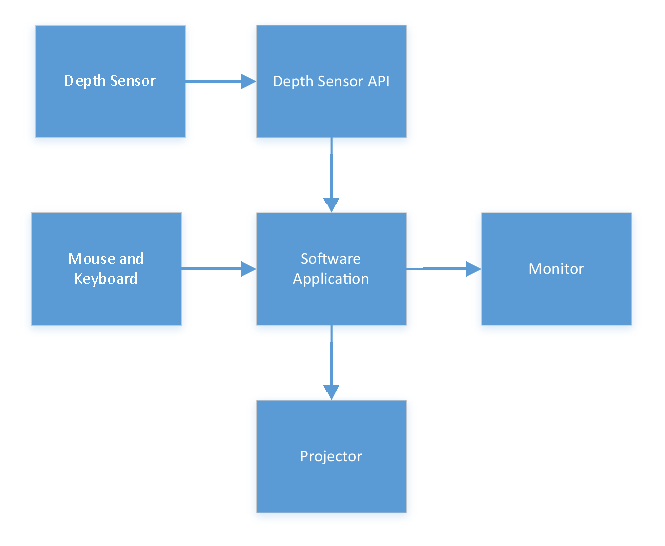
\includegraphics[width=6in]{BlockDiagram}
    \caption{An overview of the system's components and how they interact}
    \label{fig:overview}
\end{figure}

%-----------------------------------------------
% Maybe have more higher level paragraphs explaining the modes and what they do
% As opposed to the low-level list of stimuli and reactions
%-----------------------------------------------

\subsubsection{System Modes}
\begin{enumerate}
\item{Calibration Mode}
Calibration mode is used to calibrate the depth sensor and projector, mainly for use during the initial set\-up process for the sandbox. A summary of features is listed below:

\begin{itemize}
\item \textbf{User switches to Calibration Mode}
Current bounds of the projection area are shown on the sand.

\item \textbf{User uses the computer terminal to adjust bounds of projection area}
A bounding box appears when the mouse is moved, this box dictates the area defined as the sandbox.

\item \textbf{User calibrates depth sensor by placing an object with flat sides on the sand}
Using height sensor data, the outline of the object is projected onto the sand. 
The computer terminal is used to move this outline around until it lines up with the physical object.

\item \textbf{User changes the current display mode}
The current display information shall be replaced with the information that corresponds to the display mode selected.
\end{itemize}

\item{Depth Mode}
While in Depth Mode, the program will visually represent the height of the sand using color and contour lines. Below is an overview of Depth Mode's features:

\begin{itemize}
\item \textbf{User observes sandbox}
The different heights at different points along the surface of the sand shall be visually represented via a projection.  This projection will consist of a 2-dimensional representation of the height projected onto the 3-dimensional surface of the sand.

\item \textbf{User physically manipulates the sand, changing the landscape in the box}
The visual representation projected on the sand shall adjust in accordance to the new height of the sand in the areas that have been altered. 

\end{itemize}

\item{Design Mode}
Design mode is used to control the shape of the road segment that is projected onto the terrain. A summary of features is listed below:

\begin{itemize}
\item \textbf{User switches to Design Mode}
A segment of road is displayed.

\item \textbf{User uses the computer terminal to edit the path of the road}
The user shall be able to adjust the position and curvature of the road.
The user shall be able to place additional manipulation points along the road which can be used to further refine the path of the road.
A edit/reset button shall be present to revert the road back to its previous path.
The User shall be able to undo unwanted changes.

\end{itemize}

\item{Cut \& Fill Mode}
Cut and Fill mode is used to visualize the volumes of material that must be added or removed in order to achieve the desired road path. A summary of this mode's features is outlined below:

\begin{itemize}
\item \textbf{User observes sandbox}
A road shall be displayed traversing the surface of the sand.  Along this road, the amount of sand that would be required to be taken away or put in place in order to achieve the desired alignments along the road shall be visually represented.  In addition, the total haul quantity, average haul distance, average haul grade, estimated haul duration, and the construction equipment to use shall be displayed.

\item \textbf{User physically manipulates the sand, changing the landscape in the box}
The representation along the road and the additional information described above shall adjust in accordance to the new height of the sand.
\end{itemize}
\end{enumerate}
%---------------------------------
% May want to reorganize these subsections.  Just need to cover all bases, how we organize is up to us.
%Also, this is a rough draft, so no matter if we miss a few things.
%---------------------------------
\subsection{System Architecture}
%Provide a model for our solution
%What is going to make up the system described above?
The purpose of this subsection is to provide the model of our AR Sandbox System.  
The Architectural Design subsubsection demonstrates how this system is comprised of various components which interact with one another; these relationships and interactions are explained and displayed with diagrams and figures. 
The Decomposition Description subsubsection goes into further detail about each of these components and how they are implemented.
Lastly, the Design Rationale subsubsection provides reasoning behind some of the design choices presented previously.

\subsubsection{Architectural Design}
\par Figure 2 gives an overview of the software architecture and shows how the different components, such as the heightmap and vertex/fragment shader takes the input from the depth sensor and renders it into a terrain mesh.



\begin{figure}[H]
	\centering
	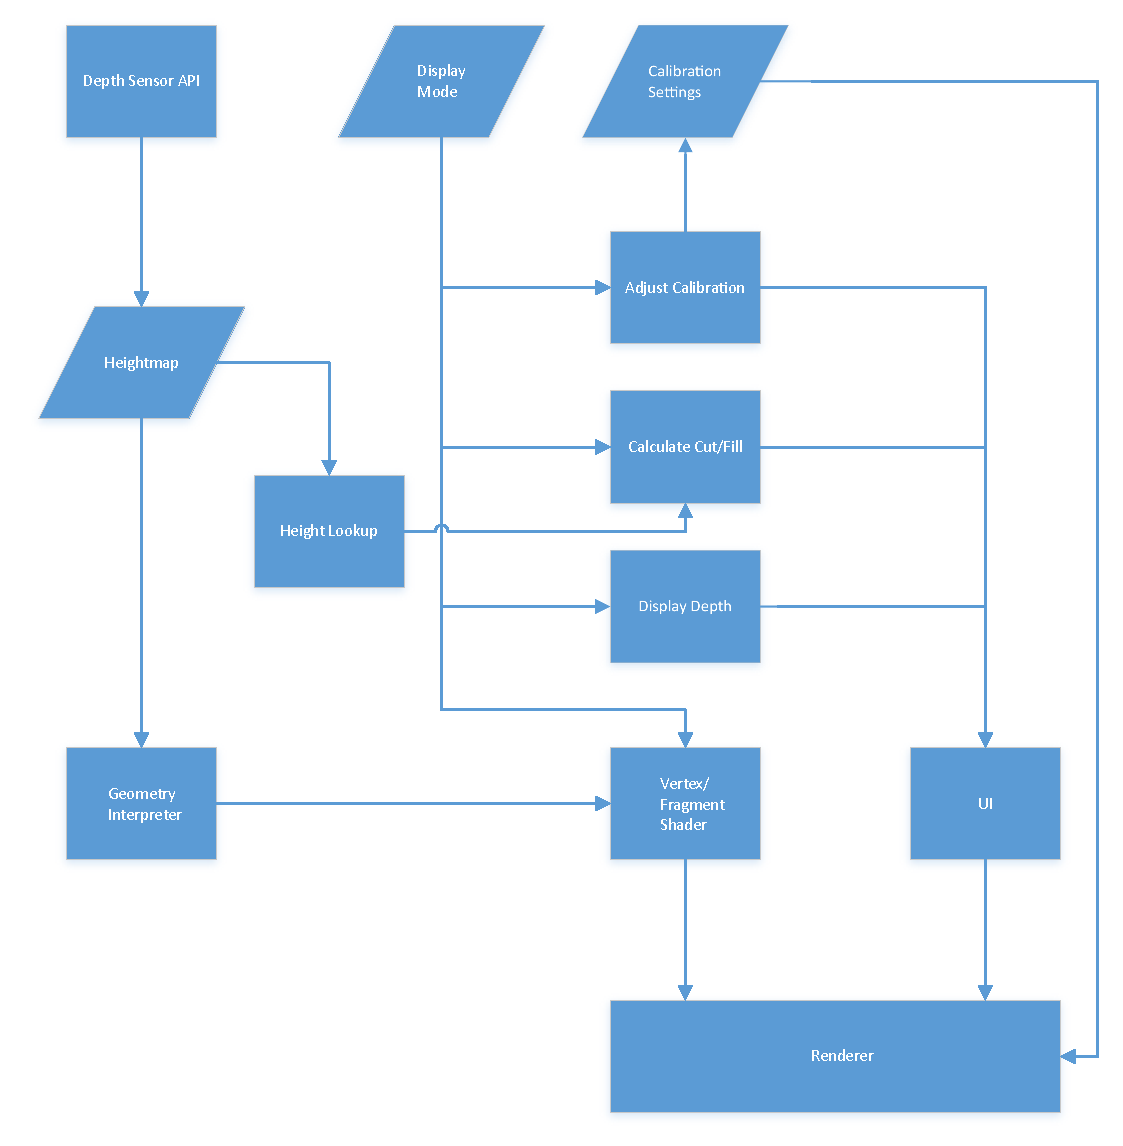
\includegraphics[width=6in]{SysArch}
    \label{fig:sysarchitecture}
\end{figure}

\begin{figure}[H]
	\centering
	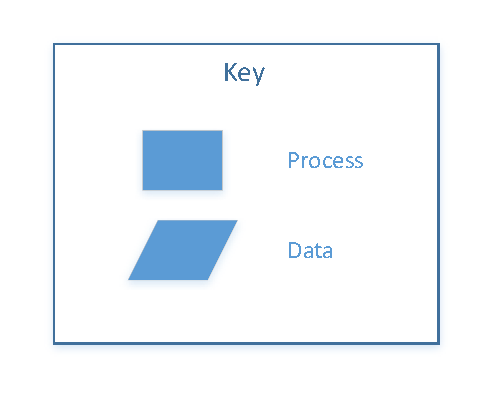
\includegraphics[width=2in]{SysArchKey}
    \caption{System Architecture}
\end{figure}

%\subsubsection{Decomposition Description}
%Talk about the nodes described in Arch. Design. 
\begin{enumerate}
\item{Depth Sensor API} %Mark

The Kinect's API allows for the Kinect sensor to interface with the rest of the sandbox system.
It provides access to the sensor's depth image data, raw infrared image, full-color image, and has built-in body tracking functionality \citeDesign{kinect_api_overview}.
For this system, the API's primary functionality will be providing the sensor's depth image data which will be stored as the heightmap.


\item{Geometry Interpreter} %Andrew
The Geometry Interpreter takes the heightmap data from the depth sensor and converts it into a three dimensional mesh.
It is responsible for performing any downsampling required to make the mesh renderable in real time.

\item{Height Lookup}
The height lookup module is responsible for fulfilling requests for height data at a given point on the terrain mesh.
This is accomplished by correlating the point in 3-space to a pixel on the heightmap, and multiplying the resulting greyscale (normalized to 1) value by the maximum height of the terrain.

\item{Adjust Calibration} %Mark
Adjust Calibration is used to adjust system settings in order to ensure the sensor and projector are properly aligned with each other as well as the surface of the sand.  
These setting include adjustments in area the depth sensor is looking in and the area covered by the projection.
This module continually interacts with the UI as it prompts the user with the setting to be adjusted and then stores these settings in the Calibration Settings.

\item{Calculate Cut/Fill} %Raja
Cut and fill refers to the process of creating a level path where a road or highway can be built.
The cut or fill of a road will be calculated by determining the height of a part of the sand where the road should be, then displaying a colored view of the road.
For example, if the road is below a certain height, the it's displayed using a shade of blue.
If it's above a certain height, the road is displayed using a shade of red.

\item{Display Depth} %Raja
Display depth is used to visualize the height or altitude of an area.
If a part of the sand is above a certain height, then it's displayed using a shade of red.
If the sand is below a certain height, then is displayed using a shade of blue.
The intensity of the color depends on how far the height of the sand is from a predetermined height.

\item{Vertex/Fragment Shader} %Andrew
This program utilizes two pairs of vertex and fragment shaders written in the OpenGL Shader Language (GLSL). 
The first is responsible for coloring the terrain mesh in order to visually represent height information. 
The second is used to color road segments to represent cut and fill data. 
The visual appearance of these shaders will change depending on the current display mode.

\item{User Interface} %Raja
The user interface allows the user to manipulate the design of the road or change the display mode.
The user will interface with the software via a standard computer terminal with a mouse and keyboard.
The user can also manipulate the sand which will change the topography outputted by the software.

\item{Renderer}  %Andrew
The rendering subsystem is handled by the Unity engine, and is accessed indirectly through shaders and Unity's UI system.
\end{enumerate}

\subsubsection{Design Rationale}
%Why did we choose this design choice?
Since the software is being built using the Unity Engine, some of our design choices such as the discrete UI subsystem and choice of shader language are limited to what Unity supports. Use of a bitmap image to represent height is determined by the output of the depth sensor. 
The decision to separate different display modes into distinct modules allows for extensibility should another developer wish to add additional modes.

\subsection{Physical Architecture} %Mark
%Provide a model for our solution
%What is going to make up the system described above?


\subsubsection{Architectural Design}
Figure 3 shows the physical design of our AR sandbox.
The sandbox is a mobile box filled with sand and has an arm with a projector and depth sensor connected to an adjacent computer terminal. The components related to the physical architecture of the sandbox are described below.

\begin{figure}[H]
	\centering
	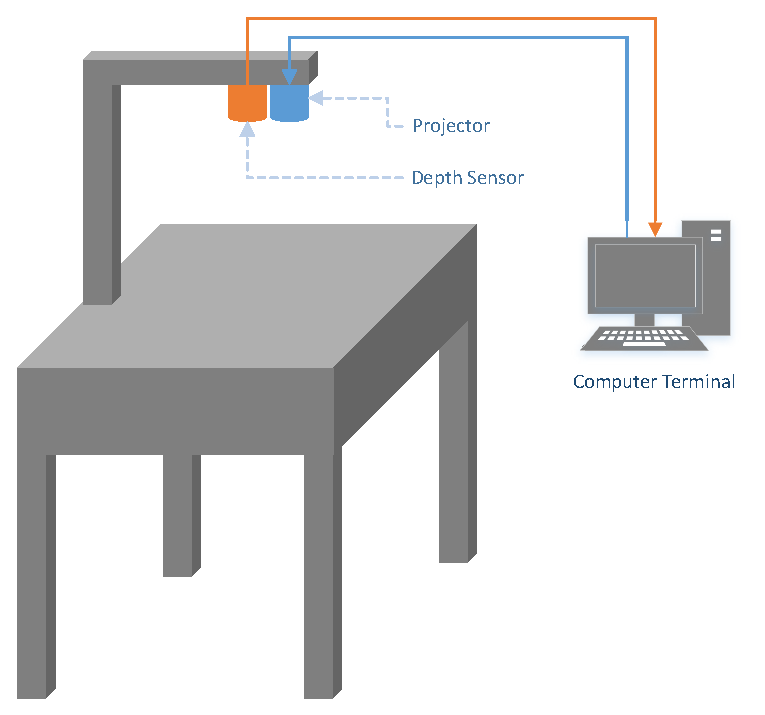
\includegraphics[width=6in]{PhysicalDiagram}
    \caption{Physical Architecture}
    \label{fig:physicalarchitecture}
\end{figure}
\begin{enumerate}
\item{Depth Sensor}

The depth sensor that will be used is a Kinect Sensor by Microsoft.  
The Kinect comes equipped with a 1280x960 full-color camera, and a Infra-Red light emitter and sensor along with an array of microphones and a tilt motor.
For this project's purposes, the Kinect's IR sensor and emitter will be primarily used and will allow us to capture a depth image.
This Infra-Red system offers a workable range of 0.8m to 3.5m from the target with a data precision of 1cm \citeDesign{andersen_jensen_lisouski_2012}.

\item{Projector}

The Projector that will be used is a AAXA M5 Mini Portable Business Projector.
This 6in X 6in X 1.8in box only weighs 1.9 pounds and offers a 1280x800p picture at 900 lumens.
Allowing for a screen up to 150in, this projector allows for a very bright and clear image for its size.


\item{Computer Terminal}
To power the AR sandbox, we will be using an HP Z240 full tower desktop computer with 16 GB of RAM, a 1TB spinning disk, and an Intel core i7 processor with a base speed of 4.2 GHz. We will install an Nvidia GTX 10XX series graphics card to handle rendering.
\end{enumerate}

\subsubsection{Design Rationale}
%Why did we choose this design choice?

When choosing the Kinect, the most important factors were the accuracy the sensor and its API.
The Kinect is one of the most accurate depth sensors on the common market and the API created by Microsoft has been created specifically for developers to use when utilizing the sensor for their applications.

The most important factors of the projector are its size/weight and its brightness.
Because of the way the projector is going to be mounted above the box, a smaller and light projector was necessary for proper stability.
With the majority of projectors at this size providing a brightness of 50-100 lumens, the 900 lumens is phenomenal.

In regards to the computer terminal, it is necessary to use a full tower desktop since a majority of graphics cards are too big to fit in a small form factor machine, or lack the hardware to mount in such a computer. Using an Nvidia GTX graphics card will give us the best results for rendering real time graphics at the lowest cost when compared to a similar workstation graphics card.

\subsection{Data Design} %Andrew
%How is the data going to flow?
%How is it stored?
This subsection discusses the specifications for the data that will be utilized by the system. The data types and methods for data storage are covered.
\subsubsection{Data Description}
The main piece of data utilized by this system is the height data received by the depth sensor API. This data is represented both as a three dimensional mesh and as a greyscale bitmap image. 
This is because the mesh must be downsampled in order to render efficiently, which, if it were the sole source of height data, would decrease the accuracy of any calculations. 
The benefit of coupling the mesh to a heightmap is twofold: first, the original data accuracy is maintained, while still reaping the benefits of improved rendering, and secondly, obtaining the height at a specific point can be made much faster since this information can be obtained through a simple texture lookup rather than through mathematical calculation.  

\subsubsection{Data Dictionary}
\begin{enumerate}
\item{Heightmap}
The heightmap is a greyscale bitmap image, in which each pixel represents a relative height. 
Each pixel is represented with 8 bits, yielding 256 shades of grey. 
In order to correlate a pixel to a y-value in 3-space, its value must be multiplied by a constant maximum terrain height. 
This is because the heightmap represents the \textit{average} height, where the lowest point is represented by a value of 0, and the highest point is represented by a value of 256.
\item{Terrain Mesh}
The terrain mesh is generated by the geometry interpreter, which converts the heightmap into a three dimensional mesh. This mesh is what is rendered by the game engine and what is colored by the shader.
\end{enumerate}

\bibliographystyleDesign{IEEEtran}
\bibliographyDesign{references}
\pagebreak

\section{Tech Review}
\subsection{Rendering Framework}
At its lowest level, the rendering framework handles the communication between an application and the graphics hardware. In this case, the term is expanded to also include game engines, which act as their own self contained development environments and handle many other tasks in addition to rendering graphics.

\subsubsection{Unreal Engine 4}
Unreal Engine is an eighth generation game engine produced by Epic Games. Notable features include real-time global illumination, full access to the engine's source code, and the ability to tweak code while the game is running in order to rapidly test features.
Unreal Engine is free to download and use, but requires 5\% of the game developer's profits upon launching their title \citeTechReview{unreal}.
The engine has a large userbase and an active forum, meaning that in-depth user created instructional content exists, and technical questions can be answered quickly. 

One of Unreal Engine's main strengths is its graphical fidelity. 
With very little effort a developer can create a realistic scene with convincing materials and lighting.
For the scope of this project however, this is irrelevant as realistic rendering is not the desired result.

\subsubsection{Unity Engine}
Unity Engine is a game engine developed by Unity Technologies. It is free to use, as long as the developer's total revenue or funding does not exceed \$100,000. Two paid versions of Unity are available, with higher revenue caps and additional features. 
Unity's scripting language is C\#, and user created shaders are specified using GLSL \citeTechReview{unity}.

One of the Unity's biggest strengths is its ability to easily deploy to multiple platforms, such as Windows, MacOS, and Linux, as well as many mobile platforms and game consoles \citeTechReview{unity}. 
This could be a boon to this project as the ability to use a computer running Linux or MacOS to create an AR sandbox could vastly increase the accessibility of our final product, as well as decrease costs for the end user.

Another strength is the relatively small learning curve. 
This makes it very easy for new developers to quickly begin creating their project in Unity, which would be beneficial to our project, given our short development period.

\subsubsection{OpenGL}
Open GL is a cross-platform computer graphics API maintained by Khronos Group. Unlike Unity or Unreal, OpenGL is not a game engine, but instead an interface between an application and the GPU. This means that OpenGL does not provide a development environment, or specify that a particular language be used to develop the application. 

The main benefit of using OpenGL is performance, since no additional features are provided, there is no overhead for features that go unused. The developer is free to specify exactly what they want the graphics hardware to do without interfacing with an additional layer of abstraction, such as a game engine. This can also be a drawback as one of the main draws to using a game engine is the ease of development and the fact that the engine automatically takes care of much of the heavy lifting associated with rendering an object on the screen. 

For a project such as this, the majority of a game engine's features such as physics will go unused, and a majority of the rendering power built in to the engine will be either turned off or hidden, making a much lower level system such as OpenGL more attractive. 

\subsubsection{Conclusion}
While the more efficient OpenGL is certainly an attractive choice for this project, the best tool for the job is the Unity engine. Unity provides a middle ground between Unreal 4, which is focused more on photorealistic rendering, and the simplicity of OpenGL. Unity retains all the integrated build support of a game engine while still being easy to use and fully capable of supporting the requirements of this project. While we may gain additional performance from OpenGL, Unity's performance should be more than acceptable for the caliber of graphics that we wish to achieve. 

\subsection{Height Data Storage}
In order to save the sandbox's topology, a digital representation must be created. This representation must contain enough information to correctly recreate the sand's surface.

\subsubsection{Greyscale Bitmap}
The most logical option for storing the terrain of the sandbox is with a greyscale bitmap image, since this is the format that the depth sensor uses to express this information. The benefit of this approach is that a bitmap is relatively small in comparison to other options, and represents all the information required to recreate the sand's surface, without additional unnecessary metadata. The main downside of this approach is that if the user wishes to reconstruct the sand's surface in an easy to visualize manner, they will have to convert the height map to a mesh. An additional downside is the fact that a heightmap is unable to represent undercuts (areas where the surface of the terrain fold back on itself, such as a cave) since it can only represent one height value per x-y coordinate.

\subsubsection{FBX File Format}
The FBX file format is a proprietary file format designed by Autodesk for storing three dimensional scenes. The FBX format is one of the most widely used 3D file formats because of its ability to also store additional scene data such as camera position, skeletal meshes used for animation, lights, and materials, as well as its compact size. The main downside to this format is that Autodesk is not forthcoming about the structure of the FBX format, and while it does offer a C++ API which allows developers to export FBX files from their applications, the internals of this API are obfuscated. Individuals and organizations have made efforts to reverse engineer the format in order to integrate FBX import and export capabilities into a wider range of programs. Notably, Blender Foundation has been able to successfully implement FBX support into the 3D modeling package Blender without using the Autodesk provided API \citeTechReview{foundation_2013}. 

\subsubsection{OBJ File Format}
The OBJ file format was originally developed by Wavefront Technologies for use with their motion capture program Advanced Visualizer. Unlike the FBX format, OBJ files are written in plaintext, meaning that they are relatively human readable.  Another difference is that OBJ files are only capable of specifying geometry, and materials through a reference to an external MTL file. The benefit of the OBJ format is that it is supported across almost every 3D graphics platform. Another benefit is the ease of creation, since the files are written with ASCII characters \citeTechReview{reddy}. OBJ has two major drawbacks however: the first is the fact that only geometry can be stored, which for this project is a relatively minor concern. More pressing is the file size, especially when compared to the FBX format. As an example, a 6,050 triangle mesh saved as an OBJ file is 293 KB, whereas the same mesh saved as an FBX file is only 127 KB, less than half the size. Scaled up, a 732,050 triangle mesh saved as an OBJ file is 39.7 MB, and the equivalent FBX file is only 11.9 MB. 

\subsubsection{Conclusion}
The best approach for storing height data is to use a greyscale heightmap, with the option of exporting an OBJ file should the user request one. An image file is far more compact than any of the 3D file formats discussed and contains all the information necessary to recreate the sand's topology. The only downside is that it's less meaningful than viewing an actual three dimensional mesh of the terrain; a downside mitigate by giving the user the option to export one. The OBJ file format is preferable due to its ease of creation and universal support.

\subsection{Height Data Representation}
Raw data from the AR sandbox's depth sensor takes the form of a heightmap - a greyscale image whose pixels correspond to the height of the sand at a specific location. The heightmap must be interpreted by our application in order to display meaningful information on the sand. 

\subsubsection{Two Dimensional Representation}
One approach is to use the value at each pixel in the heightmap to color pixels on a 2D image in order to represent height. 
The benefit of this technique is simplicity, as there is only one step involved in converting raw height data to the final image. 
A drawback to this approach is that it offers little flexibility should we or another developer wish to implement additional features in the future.

\subsubsection{Three Dimensional Representation}
Another approach is to use the height data to generate a three dimensional mesh. A shader would then be used to apply color to the mesh to represent the height. A top-down view of this mesh would then be projected onto the sand. While this seems like unnecessary work and does add an extra step to the rendering process, it gives us a lot more flexibility when adding additional features. For instance, when simulating the effects of runoff on the terrain, the mesh could be used to calculate the flow of water. Additionally, if the user wants to save the state of the sandbox, having a three dimensional representation of the topography at a specific time would give the saved data more meaning as the user would be able to view not only the path of the road, but also the terrain that the road is passing through. 

One downside to this approach is the additional computational cost of looking up the height of individual points. If using a mesh, it is first necessary to determine which triangle the point falls on, then use the three vertices that make it up to determine the height of the point geometrically.

Another downside is that, depending on the resolution of the heightmap, the resolution of the three dimensional mesh may need to be downsampled in order to efficiently render the mesh.

\subsubsection{Coupled Two and Three Dimensional Representation}
A third option is to retain both the original greyscale heightmap, as well as render a three dimensional mesh. While this would be the most computationally expensive approach and would require more data to be stored in RAM, it would be very easy to obtain the height value at a given point. The point in three dimensional space would need to be correlated to a pixel on the heightmap, which could then be sampled to get a height value. This approach also mitigates the issue of having a lower resolution mesh than the original heightmap since the original heightmap is maintained and can be referenced when exact heights are required.

\subsubsection{Conclusion}
Maintaining both a mesh and a heightmap is the best approach as the additional computational overhead imposed would be more than made up for by the ease of acquiring height information. Additional RAM usage is not a major concern either as the capacity of modern memory modules is so large. The ability to render a lower resolution mesh would also be helpful since even a low resolution heightmap would require a large number of triangles to represent it at full resolution. As an example, a 480 by 480 pixel heightmap would require \[ \frac{480^2}{2}=115,200 \] triangles to be rendered. While not implausible with modern graphics hardware, this could be a concern for older computers.

\subsection{Depth Visualization}
\subsubsection{Overview}
Depth visualization consists of ways of interpreting the height or depth of a landscape or feature.
It is a method of scientific visualization and, as an example, can be used to model or visualize the terrain of a geographic area.
For our project, the feature being visualized is the height or depth of sand in a sandbox.

\subsubsection{Criteria}
The depth of the sand must conveniently communicate to the user the lay of the land or, more specifically, the altitude or elevation of an area.
This can be done effectively using technologies such as a color map, a contour map, or a topographic map.

\subsubsection{Potential Choices}
\begin{enumerate}
\item{Color Map}
Color is a convenient and easy way of modeling data and allows people to quickly understand a complex system or environment.
"Digital elevation data can be translated into many types of terrain displays and maps, including color-scaled contour maps...conventional contour maps, and shaded relief maps."\citeTechReview{tech:1}
Therefore, our first choice for representing height would be a color map.
This color map would use different colors to represent the height or altitude on the map.
For example, land at sea level would be blue while land above sea level would be green.
Land at a high altitude would be represented in yellow or red indicating hills or mountains respectively.

\item{Contour Map}
A classic method of representing terrain elevation is a contour map.
The typical contour map uses successive contour lines to represent altitude.
Features of the landscape, such as hills or mountains are outlined using these contour lines.
These contours can be used to give an outline of the terrain.

\item{Topographic Map}
Topographic maps can be thought of as a combination of both color and contour maps.
"Topographic maps are a detailed record of a land area, giving geographic positions and elevations for both natural and man-made features"\citeTechReview{tech:2}.
In addition, topographic maps are also traditionally used in highway planning, because they provide important information "about the features of the land, approximate amount of cut and fill, drainage, where bridges may be needed, degree of economic development of the area, and other useful information".\citeTechReview{tech:2}
This makes topographic maps an excellent choice for visualizing depth, because it is a format that civil and construction engineers would be familiar with.
\end{enumerate}
\subsubsection{Discussion}
While both the color map and contour map can be used to represent the same thing, color is an easier indicator of height or altitude when compared to contour maps, since contours in a contour map need to be counted.
Contrast this with easily looking at the color of an area and recognizing the elevation.
However, topographic maps combine both of these advantages and therefore provide both means of reading the terrain.
On top of this, topographic maps are a more traditional format that civil and construction engineers would be familiar with.

\subsubsection{Conclusion}
A topographic map may be the best choice, simply because it can represent more information than a color or contour map.
Additionally, topographic maps are already used in fields such as civil engineering and city planning.

\subsection{Cut and Fill Visualization}
\subsubsection{Overview}
Cut and fill refers to the process of creating a level path where a road or highway can be built.
Visualizing the cut and fill of a road helps engineers determine the amount of earth that will need to be moved in order to create a level roadway.
Land that is too high in elevation is cut and land that is too low in elevation is filled.

\subsubsection{Criteria}
The cut and fill of a road must be easily determined simply by looking at the road itself or looking at some sort of diagram representing the road.
This is a key feature of our project and must be intuitive enough that the engineer can tell which part of the road will need to be cut and which part will need to be filled.

\subsubsection{Potential Choices}
\begin{enumerate}
\item{Color}
An easy and simple way of visualizing the cut and fill of a road is using a color coordinated system similar to the topographic map.
For example, an area that needs to be filled is colored blue and an area that needs to be cut is colored red. 

\item{Mass Haul Diagram}
Another way of visualizing cut and fill is using a mass haul diagram.
A mass haul diagram is "a graphical representation of the cumulative amount of earthwork moved...and distances over which the earth and materials are to be transported."\citeTechReview{tech:3}
The y-axis of a mass haul diagram represents the volume of material to be cut or filled, while the x-axis shows the distances the material will need to be hauled.

\item{Cut and Fill Table}
A table can also be used to show cut and fill for a road.
Each subsection of the road could be represented by a positive number showing the amount to fill, while a negative number could represent the amount to cut.
This would look similar to an Excel spreadsheet.
\end{enumerate}
\subsubsection{Discussion}
The cut and fill table would not be a good choice, because it does not effectively convey the cut and fill of the road in an easy manner.
The user would have to analyze the numbers in the table and mentally visualize the cut and fill.
In contrast, the mass haul diagram is commonly used when building roads and highways and conveys the necessary information graphically; however, when talking with our client, he mentioned that the mass haul diagram can be confusing since it requires showing both the profile of the road and a graph of the cut/fill volume.
An easier method may be representing cut and fill using a color map.

\subsubsection{Conclusion}
The best way to represent the cut and fill would be using color.
Color would allow the user to simply eyeball the road and make a determination if the subsection needs to be cut or filled.
Higher gradations or intensities of color can show if more earth needs to be cut or more filled.

\subsection{User Interface}
\subsubsection{Overview}
For our project, the user will be able to manipulate the design of the road and change the display mode of the augmented reality sandbox.
It's important that the user interface is organized in a convenient and simple way in order to make the user comfortable.

\subsubsection{Criteria}
The user interface must be in a format that is familiar to the user, but also useful enough to utilize the software.
The cost of input devices for the user interface as well as whether the user will need to be trained to use the software is another requirement to consider.

\subsubsection{Potential Choices}
\begin{enumerate}
\item{Computer Terminal}
Our first choice would be to use a simple keyboard and mouse interface on a computer terminal.
A majority of software programs are used with a mouse and keyboard so this would be something a user would more than likely be familiar with.

\item{Projected UI}
Our client discussed the possibility of using some sort of hardware pointing device to manipulate the road design and interact with UI elements.
A similar project I found shows a proof of concept using a Wii Remote.\citeTechReview{tech:4}
This would basically be a windows interface, but projected on the sand.
This would make it easier for users to see what they're doing and get instant feedback.

\item{Gesture Controls}
Another choice brought up by our client is using a gesture based interface.
Certain gestures would be captured by the hardware and interpreted as interacting with the software.
I came across a project demonstrating a proof of concept of this idea, again using a Wii Remote.\citeTechReview{tech:5}
This is a novel method and unlike the projected UI would not require the use of additional hardware, since we will be using a Microsoft Kinect as a depth sensor.
The Kinect could also be used to track a user's hands.
\end{enumerate}

\subsubsection{Discussion}
The gesture control interface is an interesting and novel idea; however, it may be too confusing for users who are used to a more simple keyboard and mouse interface.
Users may need to be trained before they can use gestures. In contrast, the projected UI would be intuitive, as it would be similar to a basic windows interface, but projected onto the sand.
However, this technology may incur extra costs since we would need to implement some sort of hardware pointing device.
On top of that we would also need to learn how to interface the new hardware with our software.
The interface projected on the sand may work, but it may simply be easier to use a computer terminal that users most likely have experience with.

\subsubsection{Conclusion}
The computer terminal interface would be our choice, because it's a technology that user's are familiar with and would not require additional training or cost to use or implement.

\subsection{Capture of Data}
\subsubsection{Overview}
In order for the system to properly represent the height of the sand via projection, it has to capture the height of the sand as input.
This can be done in several different ways: with the use of scales recording the weight of the sand atop it; a camera recording the surface of the sand and extrapolating the height from that; or a 3-dimensional depth sensor to take in the heights at various points.
\subsubsection{Criteria}
All of the potential choices have positives and negatives.
In order to make the best decision, the following will be used as the primary criteria which will be used to assess the various options.
These criteria include the following:
\begin{itemize}
\item Precision: How precise the measurements taken are.
\item Cost: How much it is going to cost to implement.
\item Data Manipulation: How much the raw data must be manipulated in order to achieve the desired information.
\end{itemize}

\subsubsection{Potential Choices}

This subsection explores three potential choices for how the system can capture the height of the sand throughout the sandbox as input.
The first of these choice is the installment of a grid of scales along the floor of the sandbox, measuring the amount of sand above that given point.
The second choice is to utilize two cameras positioned above the sandbox, creating a stereoscopic image for the system to analyze.
The final option is to utilize a 3-dimensional, depth sensing camera placed above the sandbox.  

\subsubsection{Discussion}

The greatest drawback when using scales to determine the height of the sand is the lack of precision.
A scale will only ever yield the average height along the area that it is weighing.
With smaller scales, comes a greater quantity needed in order to fill the area of the sandbox, and a sharp increase in cost.
With most scales costing around \$100, the cost of creating a grid would get very expensive very quickly \citeTechReview{scales_galore}.
In addition to the high costs and lack of precision, using scales also requires a increased amount of data manipulation.
The data captured via the scales is the weight of the sand placed atop it.
In order to get the desired height data, that weight must be manipulated using the density of sand and the area the scale covers in order to get the average height within the area.
This is far from efficient and will require a vast number of calculation.
\\\\
Utilizing two different cameras to capture a stereoscopic view is more precise than using scales to measure the sand's weight.  
It depends on the resolution of the camera, but instead of just providing the average height over larger areas, the cameras can provide a height for a given point along the surface of the sand.
In addition to the increased precision, it is also slightly more cost efficient.
These days, computer interfacing cameras can be purchased for as cheap as \$10 \citeTechReview{amazon}.
By having two cameras record the state of the sand, we create a system that acts much like the human eyeballs. 
By analyzing the disparity between the a point from one camera to another the height of that point is able to be derived \citeTechReview{shapiro_stockman_2001}.
Because of the increased precision, more calculations have to executed in order to complete the data, and those calculation are a lot more complex. 
Instead of an increase in cost for an increase in precision, using 2 cameras increases the amount of calculations required to manipulate the data in order to gain increased precision.
\\\\
A depth sensor yields equal (if not more) precision then a stereoscopic setup.
They often utilize similar technologies to that of the system above, but often take things a few steps further in order to improve on efficiency and precision.
A depth sensor is typically a little more expensive than using a 2 camera setup, but what it makes up for that in lack of data manipulation required.
Depth sensors are designed specifically for the task at hand.  As a result, they output the exact data needed, no additional calculations are required in order to get the various heights along the sand.

%Put in table with comparisons of criteria?

\subsubsection{Conclusion}
Of all the potential choices, it makes sense that using a depth sensor would be the best.
Depth sensors are designed specifically to provide the information that the system needs.
They have the greatest precision of all the options and the least amount of system calculations, letting the system focus on the its own calculations.
Although it is not the cheapest option available, its strengths in the other categories far outweigh the negative. 

\subsection{Depth Sensor}
\subsubsection{Overview}
The conclusion that a depth sensor is the best way for the system o gather its input begs one question: Which depth sensor should be used?
This sensor needs to be able to record the topography along the sand and send it to the system for analysis.
For the purposes of the AR Sandbox for Construction planning, the 3 of the best sensors are the Microsoft Kinect, the Intel RealSense SR300, and the Asus Xtion 2.
\subsubsection{Criteria}
In order to ensure the best possible depth sensor for the sandbox, 3 criteria have been chosen by which to compare the sensors.
These components will include the following:
\begin{itemize}
\item Quality of Camera: The quality of the camera itself.  This includes the resolution of the image taken.
\item Ease of Interface: How easy the information from the depth sensor can be sent to the computer.
\item Cost: How much the device will cost to purchase.
\end{itemize}
\subsubsection{Potential Choices}
There are three depth sensors that appear to be the best options.
The first of these is the Microsoft Kinect for Windows PC, a small sensor utilizing a infrared camera and emitter to capture depth.
The second is the Intel RealSense Camera SR300.  
The successor to the Kinect, it utilizes similar technology.
The third and final option is the Asus Xtion 2. Also using infrared to determine depth, the Xtion was created to be a direct competitor to the Kinect and RealSense.

\subsubsection{Discussion}

The Microsoft Kinect was one of the first devices to really enter the market as a infrared-using depth sensor/camera.
It emits a series of infrared beams and has a sensor to pick up the reflections and create a 3-dimensional image.
This technology and technique was found to be very accurate and only began falling off as the distance from the target was increased \citeTechReview{andersen_jensen_lisouski_2012}.
For the purposes of the sandbox, the depth sensor will be placed relatively close to the surface.
Another benefit if utilizing the Kinect is that Microsoft has already created an API in order for the sensor to interface with windows computers\citeTechReview{kinect_api_overview}.
This framework is created in order to help developers trying to utilize the sensor get going as quickly and as easily as possible.
In addition, with the age of the Kinect there is a vast amount of on line assistant available to aid in the implementation of the device.
With all of this put together, the Microsoft's Kinect costs about \$170 to purchase \citeTechReview{amazon}.
However, we already have access to a Kinect for the purposes of this project, effectively reducing its cost to \$0.
\\\\
The Intel RealSense Camera was created to be the successor to the Kinect and is encouraged to be used instead \citeTechReview{kinect_microsoft}.
The Kinect is still a used in abundance throughout the industry, but it is no longer being manufactured.
As a result, the RealSense will slowly take its place.
Being the next generation of the Kinect, the RealSense utilizes the same method for determining the depth throughout the sensor's field.
Designed to be in a depth range of 0.2 meters to 1.5 meters, the sensor fits into the exact range we need it to function within\citeTechReview{realsense_intel}.
As with the Kinect's technology, the RealSense's precision has been found to be accurate when operating within a short to medium range from the sensor\citeTechReview{andersen_jensen_lisouski_2012}.
The RealSense builds off of the Kinect's Windows interface and interacts with the computer in much the same way with its own SDK and API \citeTechReview{realsense_intel}.
In addition to these improvements to the Kinect, the Intel RealSense SR300 Camera will only cost \$109 \citeTechReview{realsense_intel}.
\\\\
The final depth sensor taken into consideration is the Asus Xtion 2.
This sensor, like the others, uses the same technology to create its 3-dimensional images.
It uses the same technology, however it does not have as strong of hardware in comparison to the Intel RealSense.
As a result, the resolution of the image taken and the precision of the data is slightly less than that of the RealSense\citeTechReview{miller_2017}.
Though there are drivers and ways for the Xtion to interface with the computer, they are not as efficient and not as well supported as that of the Kinect or RealSense.
This can partially be attributed to the Kinect being created by Microsoft and the RealSense receiving their endorsement as a device.
Bring these things together and the Xtion is less impressive than the either of the to other two sensors.
In addition, the Xtion costs \$270\citeTechReview{miller_2017}.
When comparing the abilities of the sensors and the costs, this sensor is out of the question.


\subsubsection{Conclusion}
Of all the depth sensors, the Intel RealSense appears to be the best choice when placed in a vacuum.
Both the Kinect and the Intel RealSense work a little bit better than the Asus Xtion, but the RealSense takes all that is great about the Kinect and builds upon it.
With that being said, we are not in a vacuum.
Because we already have access to a Kinect, it is the best choice for the AR Sandbox project.
Not only do we already have access to it, but it also offers a complete and accurate infra-red camera system along with a complete user API which makes the sensor particularly suited for the tasks at hand.

\subsection{Projector}
\subsubsection{Overview}
The input device has been determined, but a means of output still needed.
In order for the height visualization to be presented upon the surface of the sand, a projector is the best choice.
Projectors come in various strengths, refresh rates and costs, but which is the best for the Sandbox's purposes?

\subsubsection{Criteria}
In order to determine the best projector for the system, several aspects an option are weighed against that of the others.
These aspects include:
\begin{itemize}
\item Resolution: The resolution of the picture created by the projector.  The higher the resolution the clearer the picture projected will be.
\item Brightness: How bright the projector's bulb will be.  The brighter the bulb the brighter the environment the projection can be in.
\item Cost: How much the device will cost to purchase.
\item Size/Weight: The projector needs to be light enough to be mounted above the sandbox.
\end{itemize}
\subsubsection{Potential Choices}
The following three projectors have been determined as 3 of the best options to satisfy the needs of the Sandbox System.
The first is the ViewSonic PJD7720HD.
The second is the BenQ TH670, and the final potential choice is the AAXA M5 Mini Portable Business Projector.

\subsubsection{Discussion}
The ViewSonic projector is an all-around solid projector for its price tier.  
It offers a full 1080p picture, allowing for the data to be presented clearly to the user.
Though the picture is in full-HD, the brightness is equally important.
Without an adequate brightness, the image will not be able to be viewed at all.
The ViewSonic has a brightness of 3200 lumens, meaning the picture will be very clear in most environments.
With a cost of \$585, this is one of the better valued projectors there are \citeTechReview{best_projectors}.
With that in mind, the ViewSonic is not very compact.
It is approximately 12 in. x 9 in. x 4 in. in size and weighs 5.3 lbs; a manageable size, but not great either \citeTechReview{amazon}.

Taking a step up, the next option, the BenQ TH670, is the strongest of the projectors.
Like the ViewSonic, the BenQ projects a picture at full 1080p HD quality.
With 3000 lumens of brightness, the BenQ sits in the middle of the pack in regards to brightness.
Similar to the Epson, the BenQ allows for a screen up to 300 inches in size, overkill for what the system needs projected.
At \$700, this is by far the most expensive of the projectors.
For this price, the BenQ offers a greater screen size and built in speakers; two additions that are far from necessary in the system \citeTechReview{best_projectors}.
Along with the increased power and cost, the BenQ comes with increased size and mass.
At approximately 13 in. x 19 in. x 15 in. and weighing nine pounds, the BenQ is both larger and heaver than the ViewSonic \citeTechReview{amazon}.  
With these physical dimensions, it would be difficult the mount the projector in the desired position for the sandbox. 
\\\\
The final projector under consideration is the AAXA M5 Mini Portable Business Projector.
Once again, this projector offers 1080p HD quality.
However, the AAXA only offers 900 lumens of brightness.
This brightness will work on most low-light situations, but may begin to become hard to see when the brightness of the room starts to increase.
At a price of \$435, this is the cheapest of the options.
What the AAXA lacks in brightness it makes up in its compact size and low-weight.
It is 6 in. x 6 in. x 1.8 in. in size and weights less than two pounds. \citeTechReview{amazon}.
Though its brightness is less than that of the others, it should be noted that 900 lumens is still one of the highest available at this size of projector.
\subsubsection{Conclusion}

All 3 of the projectors discussed have their pros and cons.
They all provide a full HD picture at 1080p and adequate picture brightness for the majority of environments, with the ViewSonic providing the greatest brightness with 3200 lumens.
For BenQ projector, larger picture size is provided at a higher cost and increased size.
Because of the mounting requirements we are under and the lack of necessity for a larger picture, the BenQ is not the best projector.
The ViewSonic PJD7720HD offers a better price and smaller dimensions and weight for an unimpactful reduction of picture size.  However, its weight of five pounds is still hindersome to the mounting required.  As a result, the AAXA is the best projector for the AR Sandbox project.  It is not as bright as the others, but will be sufficient in most lighting environments, and its small, two pound body is too valuable to pass up.


\bibliographystyleTechReview{IEEEtran}
\bibliographyTechReview{references}
\pagebreak

\section{Weekly Blog Posts}
\subsection{\GroupMemberOne}
\subsubsection{Fall}
\begin{itemize}
\item Week 1
	\begin{itemize}
	\item \textbf{Plans:}
    \item \textbf{Problems:}
    \item \textbf{Progress:}
    \item \textbf{Summary:} Thought about which projects I wanted to work on. Filled out preferences. Setup OneNote and created biography. Went over resume.
	\end{itemize}
\item Week 2
	\begin{itemize}
	\item \textbf{Plans:} 
    \item \textbf{Problems:} 
    \item \textbf{Progress:} 
    \item \textbf{Summary:} Found out which project I was assigned (AR Sandbox for Construction Planning). Met with group for the first time. Emailed client and setup a time and place to meet. Scheduled time to meet with TA.
	\end{itemize}
\item Week 3
	\begin{itemize}
	\item \textbf{Plans:} 
    \item \textbf{Problems:} 
    \item \textbf{Progress:} 
    \item \textbf{Summary:} Finished and peer reviewed rough draft of problem statement. Met with client for the first time. Met with TA for the first time.
	\end{itemize}
\item Week 4
	\begin{itemize}
	\item \textbf{Plans:} Start on rough draft of requirements document.
    \item \textbf{Problems:} Final draft of problem statement due on Friday.
    \item \textbf{Progress:} Finalized problem statement and talked with team about requirements document.
    \item \textbf{Summary:} Final draft of problem statement is finished and approved. We talked about the requirements document and what we need to do. We will have to setup a meeting with the client and go over what our requirements should be for the project.
	\end{itemize}
\item Week 5
	\begin{itemize}
	\item \textbf{Plans:} Work on final draft of requirements document.
    \item \textbf{Problems:} 
    \item \textbf{Progress:} Started and finished rough draft of requirements document.
    \item \textbf{Summary:} Our team met on Tuesday after class and read over the IEEE SRS document. We started outlining the requirements document for our project. We scheduled a meeting with our client on Friday. I worked on section one of the requirements document. We went over our rough draft with the client and he gave us a lot of feedback. We scheduled another meeting with the client on Thursday next week. We'll go over the final draft of our requirements document with him then.
	\end{itemize}
\item Week 6
	\begin{itemize}
	\item \textbf{Plans:} Begin working on rough draft of the technology review assignment.
    \item \textbf{Problems:} 
    \item \textbf{Progress:} Met with client and got feedback on our requirements document. Finished the final draft of the requirements document and submitted it for client approval.
    \item \textbf{Summary:} This week, we learned about the technology review assignment. We worked on the requirements document and met with our client to get his feedback. We then worked on including his feedback in the document and submitted it for approval.
	\end{itemize}
\item Week 7
	\begin{itemize}
	\item \textbf{Plans:} Finish rough draft of technology review next week.
    \item \textbf{Problems:} 
    \item \textbf{Progress:} Started working on rough draft of tech review.
    \item \textbf{Summary:} Our team came up with nine different technologies for our project. We divided them into three technologies we each have to talk about in the technology review. I started writing the rough draft of my tech review this week.
	\end{itemize}
\item Week 8
	\begin{itemize}
	\item \textbf{Plans:} Finish final draft of technology review. Start working on design document.
    \item \textbf{Problems:} 
    \item \textbf{Progress:} Finished rough draft of tech review and started on the final draft.
    \item \textbf{Summary:} Handed in rough draft of technology review after doing peer review in class. Got good feedback on what to revise. Final draft of tech review is due next Tuesday, November 21. Our team plans on starting the design document next week, or at least talk about it. No class next week.
	\end{itemize}
\item Week 9
	\begin{itemize}
	\item \textbf{Plans:} Work on design document next week.
    \item \textbf{Problems:} 
    \item \textbf{Progress:} Finished and turned in technology review.
    \item \textbf{Summary:} Completed the final draft of the technology review and submitted it.
	\end{itemize}
\item Week 10
	\begin{itemize}
	\item \textbf{Plans:} Complete and submit fall progress report next week.
    \item \textbf{Problems:} 
    \item \textbf{Progress:} Completed preliminary design doc.
    \item \textbf{Summary:} We completed our design document and went over it with our client. He wanted certain parts revised. After revising the document, we submitted it on Friday. We will work on the fall progress report and submit that next week on Monday at 2pm.
	\end{itemize}
\end{itemize}
\subsubsection{Winter}
\begin{itemize}
\item Week 1
	\begin{itemize}
	\item \textbf{Plans:} Start work on building the AR sandbox itself.
    \item \textbf{Problems:} 
    \item \textbf{Progress:} Met with team, went over our schedules and figured out when we're all available this term.
    \item \textbf{Summary:} Met with team. We discussed our schedules and when we're available. We're all available after class on Tuesdays and can also meet up over Google Hangouts. We also discussed our plan for building the AR sandbox.
	\end{itemize}
\item Week 2
	\begin{itemize}
	\item \textbf{Plans:} Work on our design doc and tech reviews and get approval for both. Continue working on the Unity project.
    \item \textbf{Problems:} We still need our design doc and tech reviews approved.
    \item \textbf{Progress:} We worked on our documents and met with Joe this week, he went over our design doc, but he wants further revisions.
    \item \textbf{Summary:} We worked on our design document, our individual technology reviews, and we met with Joe, our client. Joe wants further revisions, but once we finish them I'm sure he'll approve our documents. Meanwhile, we talked about building the physical AR sandbox itself and Joe said that he'll purchase some components in the coming weeks. We just need to keep working on the software and get Unity working with our Kinect.
	\end{itemize}
\item Week 3
	\begin{itemize}
	\item \textbf{Plans:} Create the first version of our user interface.
    \item \textbf{Problems:} 
    \item \textbf{Progress:} Joe approved our design doc and tech reviews, which were the last documents that needed to be approved by him.
    \item \textbf{Summary:} We implemented the revisions for our design document and technology reviews that Joe wanted. We met with Joe this Friday and he approved of our documents. Now we focus on the project itself. Joe is still getting funding in order to buy the physical parts of the AR sandbox. So, we will focus on the software for now.
	\end{itemize}
\item Week 4
	\begin{itemize}
	\item \textbf{Plans:} Have the user interface implemented by Tuesday, February 6.
    \item \textbf{Problems:} 
    \item \textbf{Progress:} We created a user interface skeleton. I wrote a UI manager script that gives the buttons functionality. We'll meet on Monday and go over what is left to work on.
    \item \textbf{Summary:} We met on Monday and created a schedule of what we think should be worked on for the next month. We decided that the user interface should be the first order of business. We created a user interface skeleton. I wrote a UI manager script that gives the buttons functionality. We'll meet on Monday and go over what is left to work on.
	\end{itemize}
\item Week 5
	\begin{itemize}
	\item \textbf{Plans:} Finish project poster and midterm progress report by next week.
    \item \textbf{Problems:} 
    \item \textbf{Progress:} Finished project poster introduction and background.
    \item \textbf{Summary:}  The project poster and midterm progress report are due next week. We met up as a group on Monday and decided to split up the work. First, we'll work on the poster. When the poster is finished we'll get started on the progress report.
	\end{itemize}
\item Week 6
	\begin{itemize}
	\item \textbf{Plans:} Start work on the cut and fill mode.
    \item \textbf{Problems:} Joe wanted us to try to integrate a RealSense depth sensor into our project, but it didn't work.
    \item \textbf{Progress:} Completed rough draft of poster. Completed midterm progress report.
    \item \textbf{Summary:} We finished the rough draft of our poster and emailed it to Junki. We also completed our midterm progress report and presentation. Joe wanted us to try integrating a different depth sensor with our project, but it didn't work out. We will stick with the Kinect for now. Most of the software for our project works, but we still need to implement the cut and fill mode. We will work on that next week.
	\end{itemize}
\item Week 7
	\begin{itemize}
	\item \textbf{Plans:} Complete the cut and fill shader, or at least get close to completion.
    \item \textbf{Problems:} 
    \item \textbf{Progress:} Helped implement a design panel. This will eventually be the interface for the design mode.
    \item \textbf{Summary:} Worked more on the cut and fill shader. Implemented a design mode script that manages the design mode. Basically, clicking the design mode button opens an asset tray that will be used as the interface for creating and editing a road.
	\end{itemize}
\item Week 8
	\begin{itemize}
	\item \textbf{Plans:} Work on cut and fill calculations. Integrate features into software.
    \item \textbf{Problems:} We have separate components, now we need to integrate them.
    \item \textbf{Progress:} Finished the road shader for cut and fill mode.
    \item \textbf{Summary:} I finished the road shader for cut and fill mode. It changes the color of the road depending on whether it's above or below the terrain. I also wrote a road manager script that uses a get height function in the terrain generator to determine the height of the road above the terrain. This will make it easier to do the actual calculations for the cut and fill table. We also had a meeting with Joe today. We showed him our progress on the software and discussed how the physical sandbox will be built. Joe told us he has a guy that will build it for him. He'll probably hear back from him by next week, so we'll meet up with Joe next Friday to see how things are going. The software is basically in separate components right now. We just have to integrate it together and also hook it up to the user interface.
	\end{itemize}
\item Week 9
	\begin{itemize}
	\item \textbf{Plans:} Complete or at least mostly complete cut/fill mode.
    \item \textbf{Problems:} 
    \item \textbf{Progress:} We now get the height of the road above the terrain and display it on the cut/fill panel. Joe told us he has spoken with a technician and will meet with him on Monday. Joe also went over how to do the cut/fill calculations.
    \item \textbf{Summary:} We met with Kirsten and did our poster critique. We got a lot of good feedback which we plan on incorporating into our poster. I also worked on the cut/fill for the road. It can now display the height of the road in the cut/fill panel. We met with Joe and discussed our progress on the project. Joe told us he has spoken with a technician and will meet with him on Monday. He hopes to have a concrete timeline on when the sandbox will be built. Joe also went over how to do the cut/fill calculations and gave us some material to read over.
	\end{itemize}
\item Week 10
	\begin{itemize}
	\item \textbf{Plans:} Finish and turn in winter term progress report.
    \item \textbf{Problems:} 
    \item \textbf{Progress:} I finished up the cut and fill mode, so we have our beta release. We also met with Joe and discussed how the physical sandbox is going to be built.
    \item \textbf{Summary:} I finished up the cut/fill mode. The cut/fill panel has a table that lists out stations and each stations cut/fill information. The cut and fill is calculated based on the height of the road above or below the terrain. We also met with Joe and discussed the physical sandbox. He's picked out some parts and talked with a technician who will build the sandbox. Overall, we've finished our beta release and will work on and submit our final progress presentation for the term next week.
	\end{itemize}
\end{itemize}
\subsubsection{Spring}
\begin{itemize}
\item Week 1
	\begin{itemize}
	\item \textbf{Plans:} Meet up again on Monday at 4pm. Fix bugs in cut and fill mode.
    \item \textbf{Problems:} Many bugs that need to be fixed.
    \item \textbf{Progress:} Met with team and discussed our schedules for the term. Also went over what we have left to work on for the project.
	\item \textbf{Summary:} We had a team meeting and discussed what we have left to do. We went over what we'll need for expo, what we have left to do for our poster before submitting it, and what bugs and refinements we have left for the software. We also discussed our schedules and when we'll be available. We all agreed we could meet on Mondays and Wednesdays at 4pm. We also emailed Joe and asked if he would like to meet Monday or Wednesday next week. Lastly, we split up the tasks we have left to do. I'll focus on cut and fill mode, which is still kind of slow when performing calculations.
	\end{itemize}
\item Week 2
	\begin{itemize}
	\item \textbf{Plans:} Meet with Joe again next week. Work on the poster some more.
    \item \textbf{Problems:} Fix slow down bug in cut/fill mode.
    \item \textbf{Progress:} We met with Joe and went over how the project is going. I registered us for expo. We also worked on the poster.
    \item \textbf{Summary:} We met with Joe and showed him the progress we've made thus far on the software side of the project. He showed us how construction on the physical sandbox is progressing. So far, it's a cart with some supports for the Kinect and projector. I also registered our team for expo. We also worked on the poster this week. We reorganized poster sections so that they're easier to read, and will also work on the poster some more next week.
	\end{itemize}
\item Week 3
	\begin{itemize}
	\item \textbf{Plans:} Continue working on cut/fill mode and poster. Finish and submit Wired article assignment.
    \item \textbf{Problems:} 
    \item \textbf{Progress:} Fixed some bugs in the cut/fill mode so it fills all the columns. Worked on our poster for expo.
    \item \textbf{Summary:} I fixed some bugs in the cut/fill mode for the software so that it fills all the columns in the cut/fill panel. We had a client meeting on Monday and discussed our progress and the progress being made on the physical sandbox. We also met up on Tuesday and worked on the poster for expo. We rewrote a few sections and added some pictures so it's easier to read and look at. I also began the Wired article writing assignment. I interviewed another student and will finish my write-up by next week.
	\end{itemize}
\item Week 4
	\begin{itemize}
	\item \textbf{Plans:} Meet up with Joe on Monday and integrate the Kinect and projector with the sandbox.
    \item \textbf{Problems:} 
    \item \textbf{Progress:} Finished Wired article assignment. Finished poster.
    \item \textbf{Summary:} I finished and submitted the Wired article writing assignment. We had a client meeting with Joe and he showed us the built sandbox cart. All it needs now is sand and the projector and depth sensor mounted on it and it will be ready. We are also working on some extra features Joe requested. He wants more columns in the cut/fill mode panel so it looks like a proper cut/fill data table. He also wanted us to figure out how to graph the data so it'll display a mass haul diagram. We finished up the poster and submitted it on Canvas.
	\end{itemize}
\item Week 5
	\begin{itemize}
	\item \textbf{Plans:} Continue fixing bugs. Get sand for sandbox. Exchange projector.
    \item \textbf{Problems:} The mounting mechanism on the projector broke, so we'll need to exchange it before expo.
    \item \textbf{Progress:} Met with Joe and showed poster. Integrated projector and Kinect with sandbox. Recorded demo for report. Completed midterm report and presentation. Submitted poster and model release forms.
    \item \textbf{Summary:} Met with Joe and showed him our final poster before submitting it. Integrated the Kinect and projector with the sandbox. Currently, the sandbox is stored at the Hinsdale Wave Lab, so we have to leave before they close down for the day. I also submitted the model release forms for expo. One problem we ran into is the mounting mechanism on the projector broke, so we had to use zip ties to attach it to the sandbox. This will be sufficient for our demo, but we plan on exchanging the damaged projector for a new one before expo. We tested the system and it worked. The color changes depending on the height of an object within the boundaries of the Kinect sensor. Lastly, we recorded the demo for our midterm progress report, finished the report, recorded our presentation and submitted it.
	\end{itemize}
\item Week 6
	\begin{itemize}
	\item \textbf{Plans:} Continue working on bugs, polish things up in time for expo.
    \item \textbf{Problems:} 
    \item \textbf{Progress:} Met with Joe and discussed what we have left to do. Picked up desktop computer for sandbox. Revamped data table display.
    \item \textbf{Summary:} We met with Joe and discussed what is left for the project. We need sand for the sandbox, and this sand should be arriving by the end of the week, or possibly next week. We wanted to exchange the projector since the mounting mechanism is damaged, but Joe told us that it's passed the return window. So, we'll just have to fix the projector mounting, or improvise something come expo. We picked up the desktop computer that'll be used with the sandbox. We also went over what we have left for the software and it's mostly bug fixes and polishing things up for expo. I also implemented a revamped data table with some more columns that Joe wanted. We also had class this week and basically went over what to expect for expo and how to prepare.
	\end{itemize}
\item Week 7
	\begin{itemize}
	\item \textbf{Plans:} Work on the final report.
    \item \textbf{Problems:} 
    \item \textbf{Progress:} We had expo this week.
    \item \textbf{Summary:} We had expo this week, and it went smoothly. We spent most of the week planning out the logistics of moving the sandbox from the wave lab to Kelley. We talked with Joe, and he said that he'll have Jeff move it from the wave lab to Dearborn. Then on Friday, the day of expo, we moved the sandbox from Dearborn to Kelley.
	\end{itemize}
\item Week 8
	\begin{itemize}
	\item \textbf{Plans:} Work on final progress presentation and report.
    \item \textbf{Problems:} 
    \item \textbf{Progress:} Met up and decided we'll work on the presentation first.
    \item \textbf{Summary:} We met up this week and decided that since the presentation is due first, we should focus on that for now. We emailed Joe and will meet with him on Wednesday to hand off the project. The sandbox is being stored in Joe's office, so we will need to figure out a time when we can record a demo video with the sandbox for our presentation.
	\end{itemize}
\item Week 9
	\begin{itemize}
	\item \textbf{Plans:} Meet up on Tuesday and record demo for presentation.
    \item \textbf{Problems:}
    \item \textbf{Progress:} We continued work on the presentation and report.
    \item \textbf{Summary:} We met with Joe on Wednesday to do the project handoff. We showed how to setup the sandbox and use it. We also worked on the presentation. We will meet on Tuesday to film our demo.
	\end{itemize}
\item Week 10
	\begin{itemize}
	\item \textbf{Plans:} Finish final report.
    \item \textbf{Problems:}
    \item \textbf{Progress:} Finished final presentation.
    \item \textbf{Summary:} We finished our final presentation this week. We also worked on the final report and will finish it by Monday or Tuesday next week.
	\end{itemize}
\end{itemize}

\subsection{\GroupMemberTwo}
\subsubsection{Fall}
\begin{itemize}
\item Week 1
	\begin{itemize}
	\item \textbf{Plans:} Look at capstone projects, Submit project preferences
    \item \textbf{Problems:} None
    \item \textbf{Progress:} Looked at capstone projects, Submitted capstone preferences
    \item \textbf{Summary:} This week I investigated the available capstone projects and submitted my five preferences.
	\end{itemize}
\item Week 2
	\begin{itemize}
	\item \textbf{Plans:} Write problem statement, Schedule meeting with client
    \item \textbf{Problems:} Our client meeting was scheduled after the problem statement was due, making it difficult to write some sections.
    \item \textbf{Progress:} Wrote problem statement, Scheduled meeting with client
    \item \textbf{Summary:}
	\end{itemize}
\item Week 3
	\begin{itemize}
	\item \textbf{Plans:} Meet with client to introduce ourselves and establish project objectives, Create GitHub repo for project, Turn in problem statement, Meet with TA
    \item \textbf{Problems:} None
    \item \textbf{Progress:} Turned in problem statement, Made GitHub repo, added teammates and instructors, Met with client, Met with TA
    \item \textbf{Summary:} This week we met with our client for the first time and established what he was looking for in this project. 
	\end{itemize}
\item Week 4
	\begin{itemize}
	\item \textbf{Plans:} Meet with group to finalize Problem Statement, Email problem statement to client, Begin working on requirements document
    \item \textbf{Problems:} None
    \item \textbf{Progress:} Met with group and finished the problem statement. Problem statement was emailed to client
    \item \textbf{Summary:} This week we finished our problem statement and submitted it to our client for approval. He suggested some edits, which we added to our document before resubmitting.
	\end{itemize}
\item Week 5
	\begin{itemize}
	\item \textbf{Plans:} Meet with team to work on requirements document, Meet with client to discuss requirements document, Turn in rough draft of requirements document
    \item \textbf{Problems:} The requirements document was more involved than we originally anticipated.
    \item \textbf{Progress:} Worked on requirements document, Met with client, went over project requirements
    \item \textbf{Summary:} 
	\end{itemize}
\item Week 6
	\begin{itemize}
	\item \textbf{Plans:} Finish requirements document, Meet with client to review requirements document, Divvy up topics for tech review 
    \item \textbf{Problems:} Some of  the sections of the requirements document seem to be asking for the same thing, making it difficult to figure out what goes where.
    \item \textbf{Progress:} Finished requirements document, met with client and reviewed requirements document, made necessary changes, submitted final draft
    \item \textbf{Summary:} The majority of the week was spent finishing the requirements document, as well as thinking about what we might want to research for the technology review.
	\end{itemize}
\item Week 7
	\begin{itemize}
	\item \textbf{Plans:} Come up with tech review tasks, Divide up tech review tasks, Research tech review, Write tech review
    \item \textbf{Problems:} We didn't have class on Thursday, so we had to meet via Hangouts instead of face to face
    \item \textbf{Progress:} Came up with topics, divided up topics
    \item \textbf{Summary:} This week we focused on figuring out who was doing what for the tech review. Since this is an individual assignment, we only needed to meet as a group to discuss and divide our topics.
	\end{itemize}
\item Week 8
	\begin{itemize}
	\item \textbf{Plans:} Work on technology review
    \item \textbf{Problems:} I realized that I didn't have anything to write about for one of my sections, so I had to change topics.
    \item \textbf{Progress:} Turned in the rough draft of the tech review and received feedback
    \item \textbf{Summary:} This week I mostly focused on the tech review.
	\end{itemize}
\item Week 9
	\begin{itemize}
	\item \textbf{Plans:} Begin thinking about design document
    \item \textbf{Problems:} Being Thanksgiving week, my group was not able to meet to discuss the design document.
    \item \textbf{Progress:} I thought about the design document
    \item \textbf{Summary:} Little progress was made this week due to the Thanksgiving holiday, however I was able to review the IEEE standard for the software design document.
	\end{itemize}
\item Week 10
	\begin{itemize}
	\item \textbf{Plans:} Meet with Capstone team to discuss tech reviews/design document, Meet with client, Create graphics for the design document, Work on the design document, Finish the design document
    \item \textbf{Problems:} Being dead week, it was hard to find time to work on the design document.
    \item \textbf{Progress:} Met with Capstone team, Met with client, Finished design document
    \item \textbf{Summary:} Finishing the design document during dead week proved difficult but not impossible. We were able to meet early in the week to discuss our technology choices and again later to divvy up sections of the design document based on our research for the tech review.
	\end{itemize}
\end{itemize}
\subsubsection{Winter}
\begin{itemize}
\item Week 1
	\begin{itemize}
	\item \textbf{Plans:} Meet with team to discuss meeting times, Schedule TA meeting time
    \item \textbf{Problems:} We don't have many large blocks of time during the week that we are all able to meet
    \item \textbf{Progress:} Met with team, figured out some options for meeting times, Scheduled weekly TA meeting
    \item \textbf{Summary:} This week was mostly spent scheduling meetings
	\end{itemize}
\item Week 2
	\begin{itemize}
	\item \textbf{Plans:} Meet with team to discuss plans for the near future, Schedule meeting with client, Finish design document and tech review, Meet with client to submit design doc and tech reviews, discuss procuring equipment, Finish terrain shader
    \item \textbf{Problems:} Client currently doesn't have the funds to buy the equipment. We already have the kinect, but won't be able to get a projector for some time.
    \item \textbf{Progress:} Scheduled and met with client, planned a regular meeting time, Got feedback on design document from client, Discussed equipment procurement with client, Finished terrain shader
    \item \textbf{Summary:}
	\end{itemize}
\item Week 3
	\begin{itemize}
	\item \textbf{Plans:} Meet with client, Get approval for design document and tech reviews, Integrate Kinect into existing code, Design visual appearance of UI
    \item \textbf{Problems:} Client wants to switch to using Intel Realsense cameras instead of the Kinect. Was not able to meet with team to discuss UI designs
    \item \textbf{Progress:} Met with client, got approval for our various documents, Designed a UI, but have not had a chance to discuss it with the rest of the team
    \item \textbf{Summary:} This week I mainly worked on integrating the Kinect into our code, as well as adding some additional optimizations. Additionally, I designed a UI for our system, however I have not had a chance to review this UI with anyone else.
	\end{itemize}
\item Week 4
	\begin{itemize}
	\item \textbf{Plans:} Work on UI, Meet with client, Meet with team to make development schedule
    \item \textbf{Problems:} We got the projector we had planned on using, but the throw distance needed to get a big enough image is around 55".
    \item \textbf{Progress:} Made a lot of progress on the UI for the system. Still need to polish what we have and duplicate some menus to fully flesh it out. Made a development schedule that will take us through to the beta release. Met with client and received the projector we ordered.
    \item \textbf{Summary:} This week was spent mainly working on UI in order to prepare for the alpha release in two weeks.
	\end{itemize}
\item Week 5
	\begin{itemize}
	\item \textbf{Plans:} Finish UI, Integrate depth sensor, Start working on poster
    \item \textbf{Problems:} The depth sensor didn't arrive until Friday
    \item \textbf{Progress:} We finished the UI earlier this week, keeping us on track with our development schedule. We divided up the work for the poster and began filling in sections of it.
    \item \textbf{Summary:} This week was spent preparing for the alpha release due week 6.
	\end{itemize}
\item Week 6
	\begin{itemize}
	\item \textbf{Plans:} Finish progress report, Delegate video parts, Record videos, Finish integrating Kinect
    \item \textbf{Problems:} Some last minute bugs crept up when attempting to demo the project
    \item \textbf{Progress:} I finished integrating the Kinect, we managed to finish the progress report and video on time.
    \item \textbf{Summary:} This week we focused on the midterm progress report and attaining an alpha version for our project.
	\end{itemize}
\item Week 7
	\begin{itemize}
	\item \textbf{Plans:} Add ability to use placeholder heightmap when Kinect is not connected, Implement Bezier curves
    \item \textbf{Problems:} The Kinect API removed the ability to tell if a Kinect is connected or not.
    \item \textbf{Progress:} A placeholder heightmap is used when a private constant is switched to false. Bezier curves have been implemented, but are not controllable by the user yet.
    \item \textbf{Summary:} After finishing the progress report, this week was spent adding functionality to the system.
	\end{itemize}
\item Week 8
	\begin{itemize}
	\item \textbf{Plans:} Implement terrain manager to consolidate terrain masking and generation functionality, Add ability to modify bezier curves at runtime
    \item \textbf{Problems:} Some of the functionality in the TerrainManager class was implemented to assist with cut/fill calculations and couldn't be easily tested.
    \item \textbf{Progress:} Bezier curves can now be controlled at runtime with control points. Terrain manager has been implemented, however may require revision later as needs change.
    \item \textbf{Summary:} This week was spent refining the terrain system in order to make its architecture more congruent with the rest of the system, as well as to facilitate future additions to the system.
	\end{itemize}
\item Week 9
	\begin{itemize}
	\item \textbf{Plans:} Add visual polish, Help implement cut/fill mode, Fix issue getting height information in terrain manager, Investigate road performance issues
    \item \textbf{Problems:} I didn't have time this week to work on cut/fill mode.
    \item \textbf{Progress:} Sandbox interface now looks slightly better, terrain height lookups can be performed without raytracing, road performance is now acceptable after removing road manager script. Cut/fill mode is still not implemented.
    \item \textbf{Summary:} No new features were added this week, but existing features were improved and important bugs were fixed.
	\end{itemize}
\item Week 10
	\begin{itemize}
	\item \textbf{Plans:} Implement terrain scaling and translation in calibration mode, Implement cut/fill mode
    \item \textbf{Problems:} Cut/fill mode does a number on the performance of the sandbox.
    \item \textbf{Progress:} Cut/fill mode is implemented, however does not utilize the table in the UI yet.
    \item \textbf{Summary:} We managed to implement a rudimentary cut/fill mode this week. In order to mitigate performance issues, the mass haul is only updated every 5 seconds.
	\end{itemize}
\end{itemize}
\subsubsection{Spring}
\begin{itemize}
\item Week 1
	\begin{itemize}
	\item \textbf{Plans:} Meet with capstone team, Schedule client meeting, Work on road system
    \item \textbf{Problems:} Raja is not available Tuesdays and Thursdays, I am almost exclusively available those days
    \item \textbf{Progress:} Roads now behave as expected, height of control points can be adjusted, client meeting scheduled
	\end{itemize}
\item Week 2
	\begin{itemize}
	\item \textbf{Plans:} Work on poster, Add profile view of terrain, Write project documentation
    \item \textbf{Problems:} Profile view is slow when not using sensor data
    \item \textbf{Progress:} Worked on poster, Added terrain profile view, Started project documentation
    \item \textbf{Summary:} This week was spent creating a method for visualizing the height of the road in relation to the terrain 
	\end{itemize}
\item Week 3
	\begin{itemize}
	\item \textbf{Plans:} Polish road specification
    \item \textbf{Problems:} I did not have much time this week to work on the project
    \item \textbf{Progress:} Added lines connecting road control points making it easier to view and edit roads
    \item \textbf{Summary:} This week was spent adding additional features to design mode.
	\end{itemize}
\item Week 4
	\begin{itemize}
	\item \textbf{Plans:} Polish road specification, Finish poster
    \item \textbf{Problems:} 
    \item \textbf{Progress:} Finished and submitted poster
    \item \textbf{Summary:} This week was spent finalizing the poster for printing.
	\end{itemize}
\item Week 5
	\begin{itemize}
	\item \textbf{Plans:} Test physical sandbox, Create progress report, Record progress report presentation
    \item \textbf{Problems:} The threaded tripod mount broke on our projector
    \item \textbf{Progress:} Tested sandbox hardware, Recorded demo video, Wrote progress report
    \item \textbf{Summary:} This week we were mainly focused on getting the sandbox together and making sure everything works together, as well as recording a demo and writing the progress report.
	\end{itemize}
\item Week 6
	\begin{itemize}
	\item \textbf{Plans:} Ensure that features laid out in requirements document are met
    \item \textbf{Problems:} none 
    \item \textbf{Progress:} We were able to complete all features mentioned in the requirements document.
    \item \textbf{Summary:} This week was spent finishing small features called for in the requirements document before the code freeze on Friday.
	\end{itemize}
\item Week 7
	\begin{itemize}
	\item \textbf{Plans:} Finish visual tweaks to sandbox, attend expo
    \item \textbf{Problems:} An issue cropped up in the Get HeightAtWorldPosition function to where it was returning an incorrect height.
    \item \textbf{Progress:} Fixed GetHeightAtWorldPosition function, finished visual tweaks to sandbox, presented at expo
    \item \textbf{Summary:} The main focus of this week was preparing the project for expo, figuring out logistics, and finally presenting at expo.
	\end{itemize}
\item Week 8
	\begin{itemize}
	\item \textbf{Plans:} Begin thinking about final report and presentation
    \item \textbf{Problems:} None
    \item \textbf{Progress:} Thought about the final presentation
    \item \textbf{Summary:} This week was spent recovering from Expo and planning the final report and presentation.
	\end{itemize}
\item Week 9
	\begin{itemize}
	\item \textbf{Plans:} Meet with Joe for project handoff
    \item \textbf{Problems:} None
    \item \textbf{Progress:} Handed off the project, made plans to record demo videos next Tuesday
    \item \textbf{Summary:}
	\end{itemize}
\item Week 10
	\begin{itemize}
	\item \textbf{Plans:} Record demo video, work on final report
    \item \textbf{Problems:} We were not able to record on Tuesday, had to reschedule for Thursday
    \item \textbf{Progress:} Finished final presentation, made progress on report
    \item \textbf{Summary:} This week was spent working on the final documentation for the project
	\end{itemize}
\end{itemize}
\subsection{\GroupMemberThree}
\subsubsection{Fall}
\begin{lstlisting}
Week 1

Monday, September 25, 2017
3:41 PM

Plans:
	• Figure out which projects I would like to work on. 
	• Draft reasons why I should work on them and submit them.

Problems:
Hard to choose which projects I would like to work on.

Progress:
Figured out my preferences and submitted them.

Summary:
Throughout the week I spent most of my time trying to figure out which of the projects appealed to me.  Once I finally figured that out what projects I wanted, I wrote my reasons for why I want to work on the projects and why I would be a good candidate to work on it.  With everything done, I submitted the necessary information.

Week 2

Monday, September 25, 2017
3:41 PM

Plans:
	• Figure out what project I will be working on and contact my client and my group to figure out the best lines of communication for the future.  
	• Share this file with my TA, group members, and client.

Problems:

Progress:

Summary:
Once I figured out I would be working on the AR Sandbox for my capstone project, the first order of business was to touch bases with my group mates and figure out our lines of communication.  We exchanged phone numbers and created a group text.  After that, we touched base with our client (Joseph) and scheduled a time to meet face to face.  In addition, we decided on a time to meet with our assigned TA Junki.

Week 3

Monday, September 25, 2017
3:41 PM

Plans:
	• Meet with Joseph for the first time
	• Establish our GitHub Repo
	• Meet with Junki for the first time
	• Revise Problem Statement

Problems:

Progress:

Summary:
After meeting with Joseph for the first time, I gained a longer stronger of an understanding of what this project is going to entail and what work we are going to have to do.  In addition, we met with our TA, Junki for the first time who told us about how he will helpful to us in the future.  We created our GitHub Repo and I put my Problem Statement Rough Draft in it.

Week 4

Monday, September 25, 2017
3:41 PM

Plans:
	• Revise Problem Statement
	• Send Problem Statement Joseph for Approval
	• Get approval sent
	• Begin compiling our requirements

Problems:
	1. Joseph has some additions for the problem statement

Progress:
	1. Applied the additions and sent the changes back for approval

Summary:
This week we made several revisions to our Problem Statement and got a draft approved by Joseph.  After a little back and forth, we all came to an agreement.  In addition, we came together and agreed on our plan for next week (including what we should have ready about the requirements document by next class).

Week 5

Monday, September 25, 2017
3:41 PM

Plans:

	• Create a rough draft of the SRS and run it by Joseph to get feedback

Problems:
	1. I tried to access the IEEE document about SRS, but my access was denied.  

Progress:
	1. I tried again on a campus computer, then emailed the document to myself for use off of campus.

Summary:
This week I spent most of my time working on the SRS.  To begin, Andrew, Raja and I met up and discussed what the basic requirements were for the system and jotted them down.  We then read through the IEEE document in order to make sure we were making the document correctly.  We assigned different sections of the document to each other and split off to work on them.  I was assigned the 3rd section of the SRS, the actual requirements.  I compiled the requirements we had discussed into the document after reading through the different organizational structures and picking a combination of the Stimulus and Mode structures.  After that, I filled in as much of the rest of the 3rd section as a could prior to meeting to Joseph to go over what we had written.  We gave us extensive feedback on what we were doing correctly and what we needed to change.  These changes have been recorded and will be applied this weekend.

Week 6

Monday, September 25, 2017
3:41 PM

Plans:
	• Revise SRS into final draft
		○ Meet with Joseph about its content

Problems:

Progress:

Summary:
This week I was able to spend a lot of time working on the SRS, which proved very fortunate.  In that time, I was able to meet with Andrew and Raja several times, and both Joseph and Kirsten once.  We were able to get a lot done during these meetings and I think the SRS reflects that.  The biggest change that Kirsten mentioned was that we were being too specific in many portions of the document, be venturing into "design" territory.  Once those were taken out, the document flowed a lot better.

Week 7

Monday, September 25, 2017
3:41 PM

Plans:
	• Figure out which aspects to research for the Tech Review
	• Begin researching for Tech Review

Problems:

Progress:

Summary:

This week we began work on our tech review.  Raja, Andrew and I met up and discussed which technologies would be best to research for the sandbox and grouped them together as best we could.  We then decided who would research what.  I am in charge of researching the depth sensor, the generation/capture of data, and the projector we will use.  In addition, we met with Junki (as we do weekly) and were told that we received full points for our SRS document.

Week 8

Monday, September 25, 2017
3:41 PM

Plans:
	• Do additional work on the tech review based on the feedback from the in class peer review
	• Have the tech review mostly complete

Progress:
	• Did additional research for the Tech review, but still have a decent amount to do

Problems:
	• MECOP fall event is this week, limiting my time to work
	• Physics midterm is this week also limiting my time

Summary:
This week was incredibly chaotic and it resulted in not as much work getting done for this classes I would have liked.  I had both the MECOP fall event as well as the Physics midterm to take which severely limited my time.  I was able to put some time aside to research some more for the tech review (namely the depth sensor section), but I need to work on it a decent amount this weekend.

Week 9

Monday, September 25, 2017
3:41 PM

Plans:
Finish the Tech Review
Eat a lot of Thanksgiving turkey

Problems:

Progress:
Completed the Tech Review, unfortunately I turned it in 5 minutes late because I had trouble with my LaTeX compilation.

Summary:
This was a short week, so not a whole lot of work got done.  With that being said, a considerable amount of effort was put in during the first two days in order to turn in the best Tech Review possible using the time I had left.

Week 10

Monday, September 25, 2017
3:41 PM

Plans:
	• Create the Design Document
		○ Meet with Joseph to get okay for Document
		○ Check with his opinions on our tech review conclusions
		○ Attend Kirsten's office hours to get feedback on current design progress

Problems:
	
	• None of us really understand what the IEEE SDD document is telling us

Progress:
	• Looked at examples of Design Documents past and got a lot better grasp of what we are supposed to do

Summary:

This week was spent in its entirety to complete the design document.  I spent a lot of time both individually and with the group working on this.  In the beginning, I spent time trying to solidify my understand of what this document was asking of us, but after seeing some example I figured it out.  After that I met with Andrew and Raja several times to layout, work on, and assign sections on the document.  The design document is in a pretty place come the end of this week.  There are some known changes that are going to implemented, but there is not enough time to fully implement those within this week.

\end{lstlisting}
\subsubsection{Winter}
\begin{lstlisting}
Week 1

Monday, September 25, 2017
3:41 PM

Plans:
	• Touch base with group
	• Establish plan for near future (meeting times and such)

Problems:

Progress:

Summary:
Met with group for the first time of the term.  As a result of the meeting, we decided our scheduled meeting times would be 9am on Tuesdays and an online meeting at 5ish on Thursdays.  This will allow for stand-up like meetings to occur regularly to ensure everyone is on the same page.  We also decided meetings with Junki would be from 4:40 - 4:50 on Tuesdays.

Week 2

Monday, September 25, 2017
3:41 PM

Plans:
	• Meet with group and setup standup times
	• Meet with Joe and get orders for components in
	• Discuss how the physical sandbox is actually going to be created
	• Begin playing around with unity and getting a feel for how the program works
	

Problems:
	• I became very sick and was not able to work for a couple days
	• Joe still needs to get his funding application approved before we have the funds to get the equipment we need

Progress:

Summary:
This week, Andrew, Raja, and I met several times and discussed consistent meeting times and prepared our Tech Reviews and Design document for final approval by Joe.  We met with Joe on Friday (without me because I was sick), and got some feedback on our design document and started the discussion of ordering the components we require.

Week 3

Monday, September 25, 2017
3:41 PM

Plans:
	• Get final approval on Tech Reviews and Design Document
	• Begin work on the interfaces present within our system
	• Begin interfacing with the Kinect

Problems:

Progress:

Summary:
This week we got our Tech reviews and Design Document approved by Joe and watched several Unity tutorials to get the ball rolling on creating the interfaces for the project.

Week 4

Monday, September 25, 2017
3:41 PM

Plans:
	• Get the Interfaces of the system created in a skeletal form
	• Integrate depth sensor with Andrews mesh

Problems:
	• I have a midterm as well as my MECOP interviews this week so I will be constrained for time
	• Joe decided that he wanted to try using the Intel Realsense instead of Kinect, so we need to wait on the hardware integration until it arrives
	• Our .gitignore files isn't ignoring things properly, making version control very messy

Progress:
	• Midterms and interviews have been completed and am now able to devote more time to the project
	• Worked through .gitignore issues and got the version control a lot more clean

Summary:
This week was a stressful and very busy for me, but I feel we made some pretty good progress.  Once I got through my midterm and my interviews, I was able to start on some project things.  The team met up and we laid out a roadmap of what needed to get worked on and when we want certain pieces of the project done.  I spent a decent amount of time reconfiguring our Unity project in order to allow proper version control with it.

Week 5

Monday, September 25, 2017
3:41 PM

Plans:
	• Complete our Alpha release
	• Complete the majority of the poster rough draft
	• Complete a rough outline of our progress report

Problems:
	• The projector that we chose for the project does not have a short enough throw ratio.  As a result, the image is too small and the projector has to be moved unreasonably far in order to get  picture of sufficient size.

Progress:

Summary:
This week, we got pretty close to the Alpha release being completely done.  We only have a few touch-ups to do, but our interfaces are mainly created.  In addition, the majority of the poster was completed in a rough form.  We plan to complete the outline of the progress report this weekend.

Week 6

Monday, September 25, 2017
3:41 PM

Plans:
	• Complete the Poster template
	• Complete the progress report
	• Integrate the Kinect into the system
	• Find sufficient Projector replacement

Problems:
	

Progress:

Summary:
During this week, I spent a very large amount of time working on the progress report and poster assignments for this class.  These took a lot of time, but I feel pretty good about their quality.  There were a couple pieces of the poster (conclusions and images) which were simply placeholders at this moment, but they should be filled in in due time.

Week 7

Monday, September 25, 2017
3:41 PM

Plans:
	• We had planned to get  design mode with bezier curves complete this week, but we had not anticipated the work required for the poster and progress report last week when planning, so it might get pushed back slightly

Problems:
	1. Joe will be out of town this Friday for our usual Friday meeting
	2. Without a Kinect plugged into the system, we can't see any form of the terrain mesh

Progress:
	1. We will send out a recap email at the end of the week to keep Joe informed
	2. Create a hardcoded heightmap (like we originally had), that we can enable when working on the system without a Kinect
	

Summary:
This week I felt we got a decent amount of work complete.  Andrew was able to get the hardcoded depth image to show up when there is now Kinect present in the system which will allow me to work on things from my home computer.  In addition, I was able to create altered system behavior based on the display mode which is the first step to having the whole system and its modes link together properly.


Week 8

Monday, September 25, 2017
3:41 PM

Plans:
	• Establish draggable frame for calibration mode to decide on projections and depth sensor bounds
	

Problems:

Progress:

Summary:
I felt like I was able to get a decent amount of work done on the project this week.  My other classes had a lull in their workload and I was able to devote a lot of additional time to working on the project.  I have the framework for the Calibration window up and just need to make the TerrainMask bounds actually update when the submit button is pressed.  Waiting for Andrew's interface before proceeding their however.

Week 9

Monday, September 25, 2017
3:41 PM

Plans:
	• Complete implementation of Calibration Branch
	• Try out system with projector and Kinect to assess bugs
	• Work on adjusting the UI to look nicer
	• Do poster critique with Kirsten
	• Figure out physical sandbox status from Joe

Problems:

Progress:

Summary:
This week everything kind of came together.  I was able to complete the Calibration Mode and integrate into the master branch with it.  We did a poster critique session with Kirsten that gave us a lot of useful information about how to improve our poster and made some progress on figuring out when the physical sandbox will be available.  I still haven't been able to test the system with the Kinect and the projector myself, but Andrew has and his description has me confident.  I was unable to attend the meeting this Friday with Joe on account of me being in Portland to see my sister who was in town briefly.  In that meeting, I am told, that we discussed the Cut & Fill information that we will need to calculate and sample for the final mode of the system.  In addition to that system, we still need to make the UI look a little nicer.

Week 10

Monday, September 25, 2017
3:41 PM

Plans:
	• Finish up beta of sandbox system
		○ Complete Cut & Fill calculations
		○ Adjust the calibration window to scale terrain as well as mask

Problems:
	• Joe accidentally scheduled our meeting time in conflict with another of this meetings, so we were unable to meet

Progress:

Summary:
This week I didn't do a whole lot for the project.  We met up at the start of the week and went over the tasks to work on.  These were the completion of the Cut & Fill mode and some additional calibration scaling.  Raja said he would work on the C&F and Andrew said he would work on the Calibration.  As a result, I was just on standby most of the time, ready if someone needed me to work on something.  Because our meeting got moved to a time that conflicted with my class time, I was unable to meet with Joe this week as well.  We were able to get Cut & Fill complete, but still have some Calibration work to do.


Week 11

Monday, September 25, 2017
3:41 PM

Plans:
	• Do the final progress report
	• Record Beta level functionality video

Problems:
	• 

Progress:

Summary:
I managed to get the progress report complete and filled out the team member evaluations.
We recorded our beta level functionality video and we actually managed to get it to 28 minutes long, which I had doubts about.


\end{lstlisting}

\subsubsection{Spring}
\begin{lstlisting}
Week 1

Monday, September 25, 2017
3:41 PM

Plans:
	• Touch base with groupmates and lay out what still needs to be done
	• Touch base with Joe and see what the physical sandbox progress is

Problems:
	• I got sick for 2 days and wasn't really able to work on anything

Progress:

Summary:
This week was difficult because I got sick and was unable to get work done during that time.  I missed lecture, but Raja and Andrew got me caught up to speed.  We plan to meet with Joe on Monday.

Week 2

Monday, September 25, 2017
3:41 PM

Plans:
	• Meet with Joe
		○ Discuss what still needs to be done
		○ Show him where the software is currently at
		○ See the physical cart for the sandbox and discuss mounting rails
	• Lay out what still has to be done
	• Finish the final functionality of the calibration mode

Problems:

Progress:

Summary:
This week was pretty productive. On we met with our client and got the see the physical cart for the sandbox which really helps me to ground things mentally.  We met as a group to work on improving the poster for expo, and I was able to complete the calibration mode.

Week 3

Monday, September 25, 2017
3:41 PM

Plans:
	• Implement unit/scale feature to calibration mode
	• Revise Poster
	• Create mass-haul diagram in cut & fill mode

Problems:
	• Was sick for a day

Progress:

Summary:
	This week was spent mainly focusing on revising the expo poster and getting feedback on it.  We were able to get a lot of quality feedback from Kirsten and plan to meet again to apply that feedback next week.

Week 4

Monday, September 25, 2017
3:41 PM

Plans:
	• Figure out UI terrain mask binding
	• Complete expo poster
	

Problems:
	

Progress:

Summary:

Week 5

Monday, September 25, 2017
3:41 PM

Plans:
	• Get the Sandbox completely assembled
	• Get UI to scale properly
	• Add Scaling units
	• Get Midterm Report presentation complete

Problems:

Progress:

Summary:
A lot of time was spent this week working on this project.  The majority of that time was working to get the mounting system for the projector on the box working adequately.  After that, the time was spent filming for the demonstration in the Midterm Progress report and working on the report itself.

Week 6

Monday, September 25, 2017
3:41 PM

Plans:
	• Work on UI scaling with terrain mask
	• Double check all aspects of requirements document are checked off

Problems:

Progress:

Summary:
This week was mainly spent making sure that we had all of our requirements met before the code freeze.  I added the ability to add and remove road nodes, Andrew added the undo feature, and Raja worked on adding additional columns.

Week 7

Monday, September 25, 2017
3:41 PM

Plans:
	• Make sure that we are ready for Expo
		○ Meet with Kirsten in regards to storing the sandbox prior to Expo
	• Do Expo

Problems:
	• Need to figure out how we are storing the sandbox
	• Apparently the Expo people didn't know the dimensions of our sandbox and have moved us outside

Progress:
	• We will be bringing the sandbox over to Dearborn the say before and storing it in the Dearborn basement
	• Luckily we are in an area with tented walls to the light won't be too horrible, but need to add curtains to really see anything.

Summary:
Everything went relatively smooth during expo; the sun made it pretty hard to see, but we managed to put up some black curtains which helped a lot.  The box isn't too bad to move with sand in it, which is a nice bonus.

Week 8

Monday, September 25, 2017
3:41 PM

Plans:
	• Decompress after Expo
	• Go to class on Wednesday 
	• Discuss work that still needs to be done

Problems:

Progress:

Summary:
This week was a little lax in regards to capstone.  We did meet for our class on Wednesday and talked about everything that we still need to do for the project/class.

Week 9

Monday, September 25, 2017
3:41 PM

Plans:
	• Perform the "handoff" of the project
	• Refactor code and add comments
	• Write out changes to design and requirements document so Joe can officially approve them
	• Outline presentation recording details

Problems:

Progress:

Summary:
We performed the "handoff" with the project, which just involved us meeting with Joe and going how he can get the source code.  We me up and outlined who should do what for final presentation, and scheduled with Joe when we could come in and shoot the live-demo.

Week 10

Monday, September 25, 2017
3:41 PM

Plans:
	• Complete Final Presentation
	• Finish integrating design and requirement changes into official document to be revised
	• Complete writing of user manuals/documentation

Problems:
	• Tried to meet up to film for the presentation, but there was a scheduling conflict and we were unable to shoot

Progress:
	• We found a different time to meet that worked with everyone

Summary:
The majority of work done this week was on the presentation, as it was due on Friday.
Tuesday was spent trying to record the live-demo section, and Thursday was spent completing that recording.  Friday was then spent doing the power point piece of the presentation and splicing all the clips together for the final video.

\end{lstlisting}

\section{Final Poster}
\begin{figure}[H]
	\centering
	\includegraphics[width=6in]{poster}
    \caption{Expo Poster}
    \label{fig:expoposter}
\end{figure}

\section{Project Documentation}
\subsection{Technical Documentation}
The system is built using the Unity engine, which means that the frameworks necessary for realtime rendering are already in place. 

The main input for the system is sensor data from the Microsoft Kinect. Microsoft created a Unity plugin for interacting with the Kinect, which vastly simplified data gathering operations. Height data is received as an array of unsigned integers, which are normalized based on a known minimum and maximum sand height. Sensor data is used to generate a triangle mesh, where each index in the array represents a vertex in the mesh. A custom shader colors the mesh based on the position of each fragment in world space. We have created a number of color profiles to change the appearance of the mesh. An orthographic camera is positioned above the mesh, which captures the top-down view that will be projected back onto the sand. Since the physical sandbox has a smaller area than the field of view of the Kinect, a rectangular mask covers the terrain, making only a specified part of the terrain visible. This mask can be modified at runtime. 

The system has four modes in its current form. These modes are changed by the user through interaction with the UI, and are kept track of by a simple state machine. Each mode has its own script which listens for key presses and performs actions specific to that mode. 

\begin{figure}[H]
	\centering
	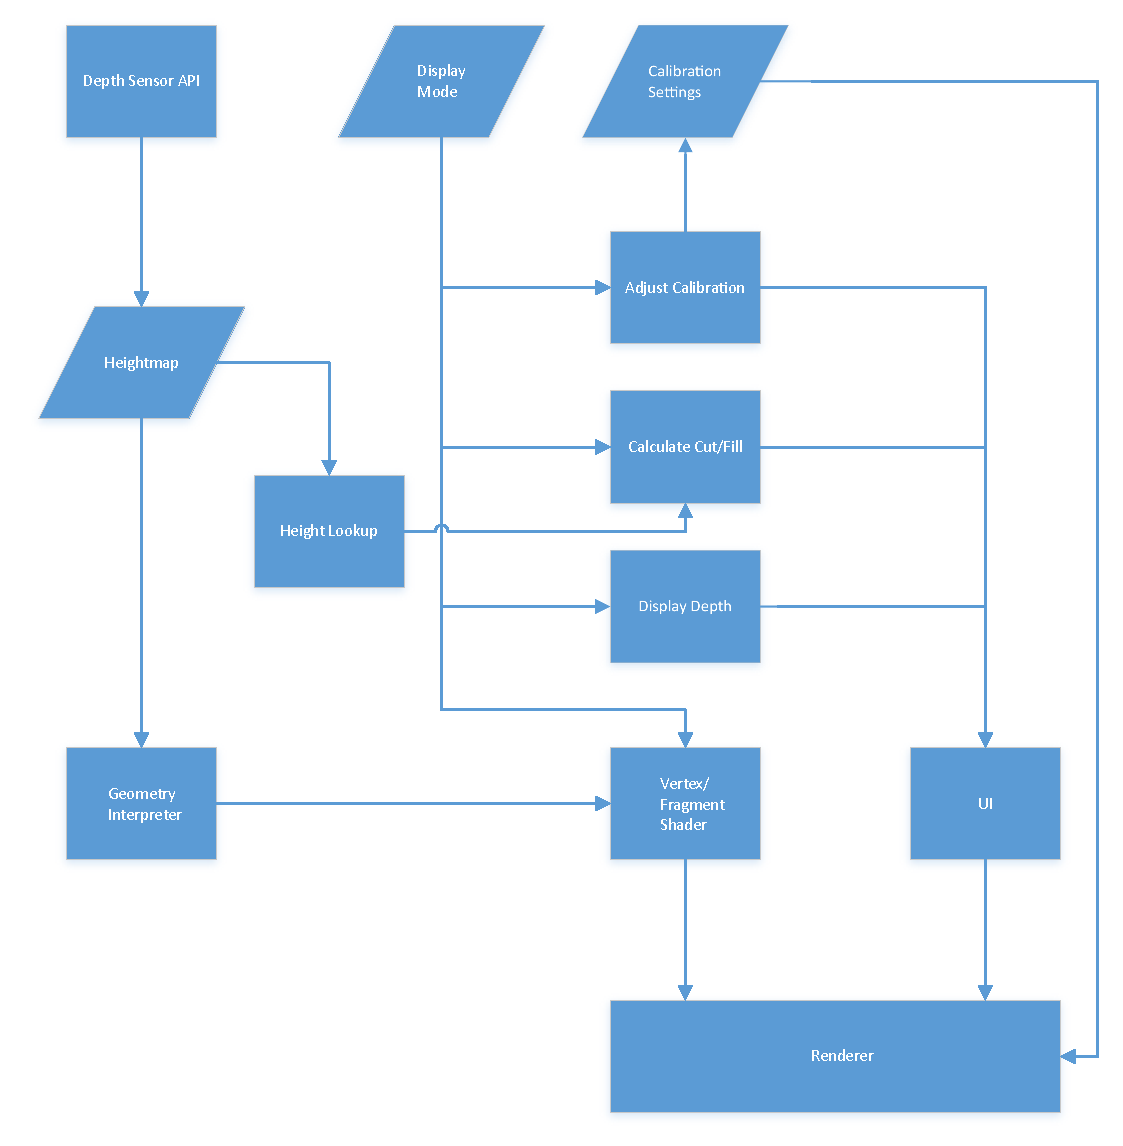
\includegraphics[width=6in]{SysArch}
    \label{fig:sysarchitecture}
\end{figure}

\begin{figure}[H]
	\centering
	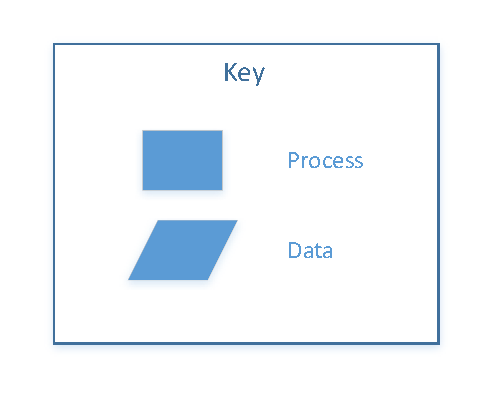
\includegraphics[width=2in]{SysArchKey}
    \caption{System Architecture}
\end{figure}

\subsection{Installation}
This project requires the Unity game engine and the Microsoft Kinect SDK to operate. After installing Unity and the Kinect SDK, run the Unity editor. Open a new project, and navigate to the src directory in the local Github repository. Unity should recognize the AR\_Sandbox directory contained in the src directory as a Unity project. After opening the project, the program can be run in editor by pressing the play button, or as an executable by navigating to File $>$ Build \& Run or pressing \texttt{CTRL + B}.
\subsection{Operation}
This section describes the different modes and details the operation of the system.
\subsubsection{Navigation}
The navigation menu is opened by pressing the \texttt{ESC} key. The menu gives the option to change mode, calibrate the system, or quit the application. The mode can also be changed by pressing \texttt{Q} for depth mode, \texttt{W} for design mode, \texttt{E} for cut and fill mode, and \texttt{R} for calibration mode.
\subsubsection{System Setup}
When the system starts, a number of parameters must be set in order to ensure proper height measurement and display. These parameters are set by opening the navigation menu and pressing Calibrate or pressing the \texttt{R} key. Begin by dragging the grey control points at each edge of the projection area so that the entire surface of the sandbox is covered by the projection. Clicking and dragging anywhere on the projection area itself will move entire projection area. To align the projected image with the physical features of the sandbox, use the Arrow Keys to translate and the \texttt{+} and \texttt{-} keys to scale it. Finally, set the lowest and highest points on the sand by adjusting the two sliders labelled maximum and minimum height that appear in the lower lefthand corner. Dig a hole in the sand down to the bottom of the sandbox, or to the desired lowest point. Build a hill to the highest desired point. Start with the Minimum Height slider at 0 and lower the Maximum Height slider until the lowest point on the sand turns red but before orange equipotential lines appear. Raise the Minimum Height slider until the highest point on the sand turns blue, but before cyan equipotential lines appear.
\subsubsection{Depth Mode}
Depth mode is used for displaying strictly the height of the sand using a color gradient. Red areas are the lowest, and blue areas are the highest.
\subsubsection{Design Mode}
Design Mode is used for designing a road segment that will be used for cut and fill calculations. When Design Mode is selected, a road will appear on the sand. This road is constrained to the bounds of the sandbox. The path of the road can be changed by clicking and dragging the orange diamond shaped control points. holding the Shift key causes a cross-sectional view of the road and terrain to appear, and allows the height of the control points to be changed by clicking and dragging with the mouse. Points can be added or removed by pressing the Add Point or Remove Point buttons. Unwanted changes to control point position can be undone by pressing \texttt{CTRL + Z}.
\subsubsection{Cut/Fill Mode}
Cut/Fill Mode is used to display a table containing information about the road segment such as cut and fill areas and volumes. When design mode is selected, the road segment will be visible. To open the cut/fill table, press the \texttt{E} key. The table updates every 5 seconds, and can be scrolled using the horizontal scrollbar to the bottom and vertical scrollbar to the right.
\subsection{Hardware}
This project requires a number of pieces of specialized hardware. At a bare minimum, a Microsoft Kinect V2, a projector, a computer with at least one USB 3.0 port, and some way to mount the Kinect and projector in close proximity are required.

\section{Recommended Technical Resources for Learning More}
\subsection{Websites}
\begin{itemize}
\item Unity API documentation (\url{https://docs.unity3d.com/ScriptReference/}): Provided information on how to utilize the Unity Game engine and greatly assisted in the speed of the project's development.
\item UC Davis AR Sandbox (\url{https://arsandbox.ucdavis.edu/}): Gave us a strong starting point and allowed us to see what a working AR sandbox should be able to accomplish.
\item Kinect API documentation (\url{https://developer.microsoft.com/en-us/windows/kinect}): Assisted in the integration of the Kinect into our system and allowed us to use it as out depth sensor.
\end{itemize}

\subsection{People}
\begin{itemize}
\item Dr. Joseph Louis (\href{mailto:joseph.louis@oregonstate.edu}{\nolinkurl{joseph.louis@oregonstate.edu} }): Client of the project, also provided us with information regarding Cut \& Fill.
\item Jeff Gent (\href{mailto:jeff.gent@oregonstate.edu}{\nolinkurl{jeff.gent@oregonstate.edu} }): Built the sandbox itself along with the cart it is mounted upon.
\end{itemize}

\section{Conclusions and Reflections}
\subsection{\GroupMemberOne}
\begin{enumerate}
\item What technical information did you learn?\\
For our project, we used the Unity game engine and the C\# programming language. Before this project I didn't have any experience with either of those technologies, so I had to spend a lot of time reading up on them and watching tutorials on Youtube. Similarly, I had to learn about civil engineering concepts such as how to calculate the cut and fill for a road, and how to read a mass haul diagram. Again, these are technical concepts I never had any experience with prior to this project. Luckily, Joe, our client was able to help me out with this and gave me some material to review, as well as answer any civil engineering related questions I had.
\item What non-technical information did you learn?\\
I learned about the logistics and paperwork involved in a large software project. Many of the documents we wrote, such as the requirements document, design documents, and technical review made me think more about the project and how to break it down. I also learned how to function as part of a team and interact with clients.
\item What have you learned about project work?\\
An important part of project work is figuring out how to break down a large project into smaller pieces that each member of the team can handle. Another important aspect is testing each of our parts of the project and then, after putting our parts of the project together, testing the whole system to make sure that each of our pieces works together.  
\item What have you learned about project management?\\
Managing time efficiently and creating some sort of roadmap to follow can greatly help when it comes to project management. There are also bottlenecks in project management. For example, there were many times where we needed a piece of hardware in order to test a function of our system, but didn't have that hardware yet. So, we had to find something else to work on in the meantime.
\item What have you learned about working in teams?\\
Working in teams presents its own challenges, but also helps because you can break down large problems into smaller, more manageable pieces. It's very important to effectively communicate with your teammates and schedule times where you can meet up. If you're not available for something, it's vital that you tell your teammates so they can make alternate arrangements.
\item If you could do it all over, what would you do differently?\\
If I could do it all over again, I would use my newfound technical knowledge to create a better software base. I learned a lot about Unity and C\# over the last year and feel that if I knew then what I know now, I would be able to implement a more efficient and better performing cut and fill software system. I would also make sure to plan things out better and anticipate bottlenecks and design changes. Lastly, there are always things that you can't control. For example, the physical sandbox wasn't built until spring term, because Joe needed to get funding for the project. In such cases, you just have to work around the problem.

\end{enumerate}
\subsection{\GroupMemberTwo}
\begin{enumerate}
\item What technical information did you learn?\\
There were two main pieces of technical knowledge I gained over the course of this project. The first is using HLSL/CG for shader specification, a shading language I was unfamiliar with prior to starting this project. Secondly, I gained a much better understanding of bezier curves, how they work, and how to implement them.

\item What non-technical information did you learn?\\
Capstone required me to interact with a a wide range of people with varying amounts of technical knowledge and investment in the project, from our client, a civil engineering domain expert with a large investment in the project, to people at expo, with a wide range of technical backgrounds and little investment in the project. Figuring out how best to talk to these people was certainly the most unique experience I gained through this project, and will certainly be applicable in the workplace. 

\item What have you learned about project work?\\
The biggest thing I learned about project work is the importance of setting smaller deadlines to break down a complex system into more manageable components. Doing so makes it much easier to divide up work among multiple people, since each person can tackle a smaller component of the larger system. Additionally it makes it easier to stay on track and gauge overall progress.

\item What have you learned about project management?\\
One important lesson I learned about project management was the importance of source control. This has been the first system I've worked on where source control is absolutely essential. At the beginning of the development process, we played fast and loose with our Git commits and as a result spent a good amount of time working through merge conflicts. Partially this was due to the way we had our Unity project set up, but mostly this was due to not communicating about what portion of the code we were working on, and not committing changes for a long period of time. After awhile we learned what works and what doesn't and had a relatively smooth source control experience for the rest of the year.

\item What have you learned about working in teams?\\
Although not something new, the importance of communication was exemplified through this project. Since we were all working on the same code base, and much of the system's functionality relies on components written by other people, communication between the three of us was essential. 

\item If you could do it all over, what would you do differently?\\
The biggest issue with this project was how late in development we actually tested our software with the physical sandbox. Luckily, everything worked together with only minor changes, but had any major issues cropped up, we would have had to scramble to fix them before expo. If we were to redo this project, I would make sure we got the details of the sandbox worked out much earlier and gotten our client to order the equipment closer to the end of Fall term instead of the middle/end of winter term.


\end{enumerate}
\subsection{\GroupMemberThree}
\begin{enumerate}
\item What technical information did you learn?\\
	The most important piece of technical information that I gained from this project is using the Unity game engine.
    Prior to this, I had never used it.
    This resulted in a relatively slow beginning, as I had to learn how to interface with the engine before I could really do any work on the project.
    In addition, I gained a better understanding of several graphical concepts through asking Andrew and Raja so that I would have an adequate understanding of how the system ticks.
\item What non-technical information did you learn?\\
	Directly interacting with a client and maintaining proper communication with them are the most important non-technical pieces that I learned.
    When working with your client (especially at the beginning of a project) it is crucial to be as open as possible in order to reduce any potential misunderstanding and prevent avoidable mistakes.
\item What have you learned about project work?\\
	As mentioned above, I learned a lot about the benefits have having proper communication with a client and making sure everyone is on the same page from the start.
    In the same vein, have a good line of communication with other team members is very important.
    This was mainly done by meeting in person as often as possible and helped to make sure that everyone was clear on the tasks at hand and who should be doing what.
\item What have you learned about project management?\\
	In regards to project management, I have learned that meeting as often as possible is vitally important.
    This helps to reduce ambiguity and makes everything clearer.
    By meeting often, we caught a lot of misunderstanding early which could have turned out to be problematic if left unchecked.
    In addition, meeting allows for everyone to be heard equally and can bring in fresh perspective on a problem someone might be having.
\item What have you learned about working in teams?\\
	When working in a team, it is vital to meet frequently and make sure everyone is on the same page.
    In addition, it is very valuable to meet early on and figure out how the assignment of work is going to happen.
    For the purposes of this class, we would meet when an assignment was given to us and create a list of all the tasks that need to be accomplished in order to finish the assignment.
    From there, it is easy to assign these tasks so that everyone has something to do and know exactly what they can work on.
\item If you could do it all over, what would you do differently?\\
	If I was to do this project again, the first big change I would make would be starting the conversation about the construction of the physical sandbox earlier.
    For a long time, we would question our client about the construction and he would say that he knew a guy who would be making it.
    In the end, they did end up making it and it turned out great.
    However, because of the time, there was a span where we had to meet very frequently in order to integrate our things onto the box.
    By starting our conversation earlier and properly pressing our client on the time sensitivity of getting the physical portion constructed, we would have had more time to work on the integration and had an easier time.

\end{enumerate}
		
\begin{appendices}
\section{Essential Code Listings}
\begin{lstlisting} [caption=The Bezier curve calculation used for specifying a road path., label=lst:bezier,captionpos=b]
	Vector3 CalculateBezier(float t, List<RoadControlPoint> points) {
		int count = points.Count;
		if (count > 2) {
			return (1 - t) * CalculateBezier(t, points.GetRange(0, count - 1)) + t * CalculateBezier(t, points.GetRange(1, count - 1));
		} else {
			return Vector3.Lerp (points [0].transform.position, points [1].transform.position, t);
		}
	}
\end{lstlisting}

The \texttt{CalculateBezier()} function takes a float \texttt{t} representing the position along the line to sample, and a list of control points that will define the line. The output of this function is a \texttt{Vector3} representing the position in world space at \texttt{t}. The function can support n control points, and works recursively to determine the position.

\begin{lstlisting} [caption=The functionality responsible for translating a Kinect height value to world space., label=lst:getheight,captionpos=b]
	public float GetHeightAtWorldPosition(Vector3 pos) {
		ushort[] heightData;
		heightData = manager.GetData ();

		Vector3 modelPos = pos - transform.position;
		Vector3 texelPos = modelPos / spacing;

		if (texelPos.x >= 0 && texelPos.x < frameWidth && texelPos.z >= 0 && texelPos.z < frameHeight) {
			float y = heightData [((int)texelPos.z) * frameWidth + ((int)texelPos.x)];
			return (((float)y - maxHeight) / (minHeight - maxHeight)) * magnitude;
		} else {
			Debug.LogError ("TerrainGenerator: Request for height data returned 0, world position out of range");
			return 0;
		}
	}
\end{lstlisting}

The \texttt{GetHeightAtWorldPosition()} function takes a world position as a \texttt{Vector3} and returns the height of the terrain at that position. This is accomplished by first converting \texttt{pos} from world coordinates to model coordinates, then determining what texel this position is associated with. Then, since height data comes from the sensor as a 1 dimensional array, the index of the texel must be determined so that its value can be returned.

\begin{lstlisting}[caption=A code snippet from the cut and fill manager demonstrating how cut and fill calculations work., label=lst:cutfill,captionpos=b]
public float[] getRoadAreas()
{
    Vector3[] positions = roadPoint.GetRoadPoints();

    float[] roadHeight = new float[roadPoint.GetNumRoadPoints()];
    float[] roadAreas = new float[roadPoint.GetNumRoadPoints()];
    int count = 0;

    foreach (Vector3 p in positions)
    {
        roadHeight[count] = 10f * terrainHeight.GetHeightAtWorldPosition(p);
        roadAreas[count] = (float)(2f * (.5 * roadHeight[count] * roadHeight[count]) + 120f * roadHeight[count]);
        count++;
    }

    return roadAreas;
}
\end{lstlisting}

The \texttt{getRoadAreas()} function returns the cut and fill areas of the road. This is done by first retrieving the points that make up the road, as shown in the \texttt{positions} array. Then, a for-each loop retrieves the height of each road point and then uses it to calculate the area. Once this is finished, the area values are stored in an array called \texttt{roadAreas} and returned to the calling function.

\section{Photos}
\begin{figure}[H]
	\centering
	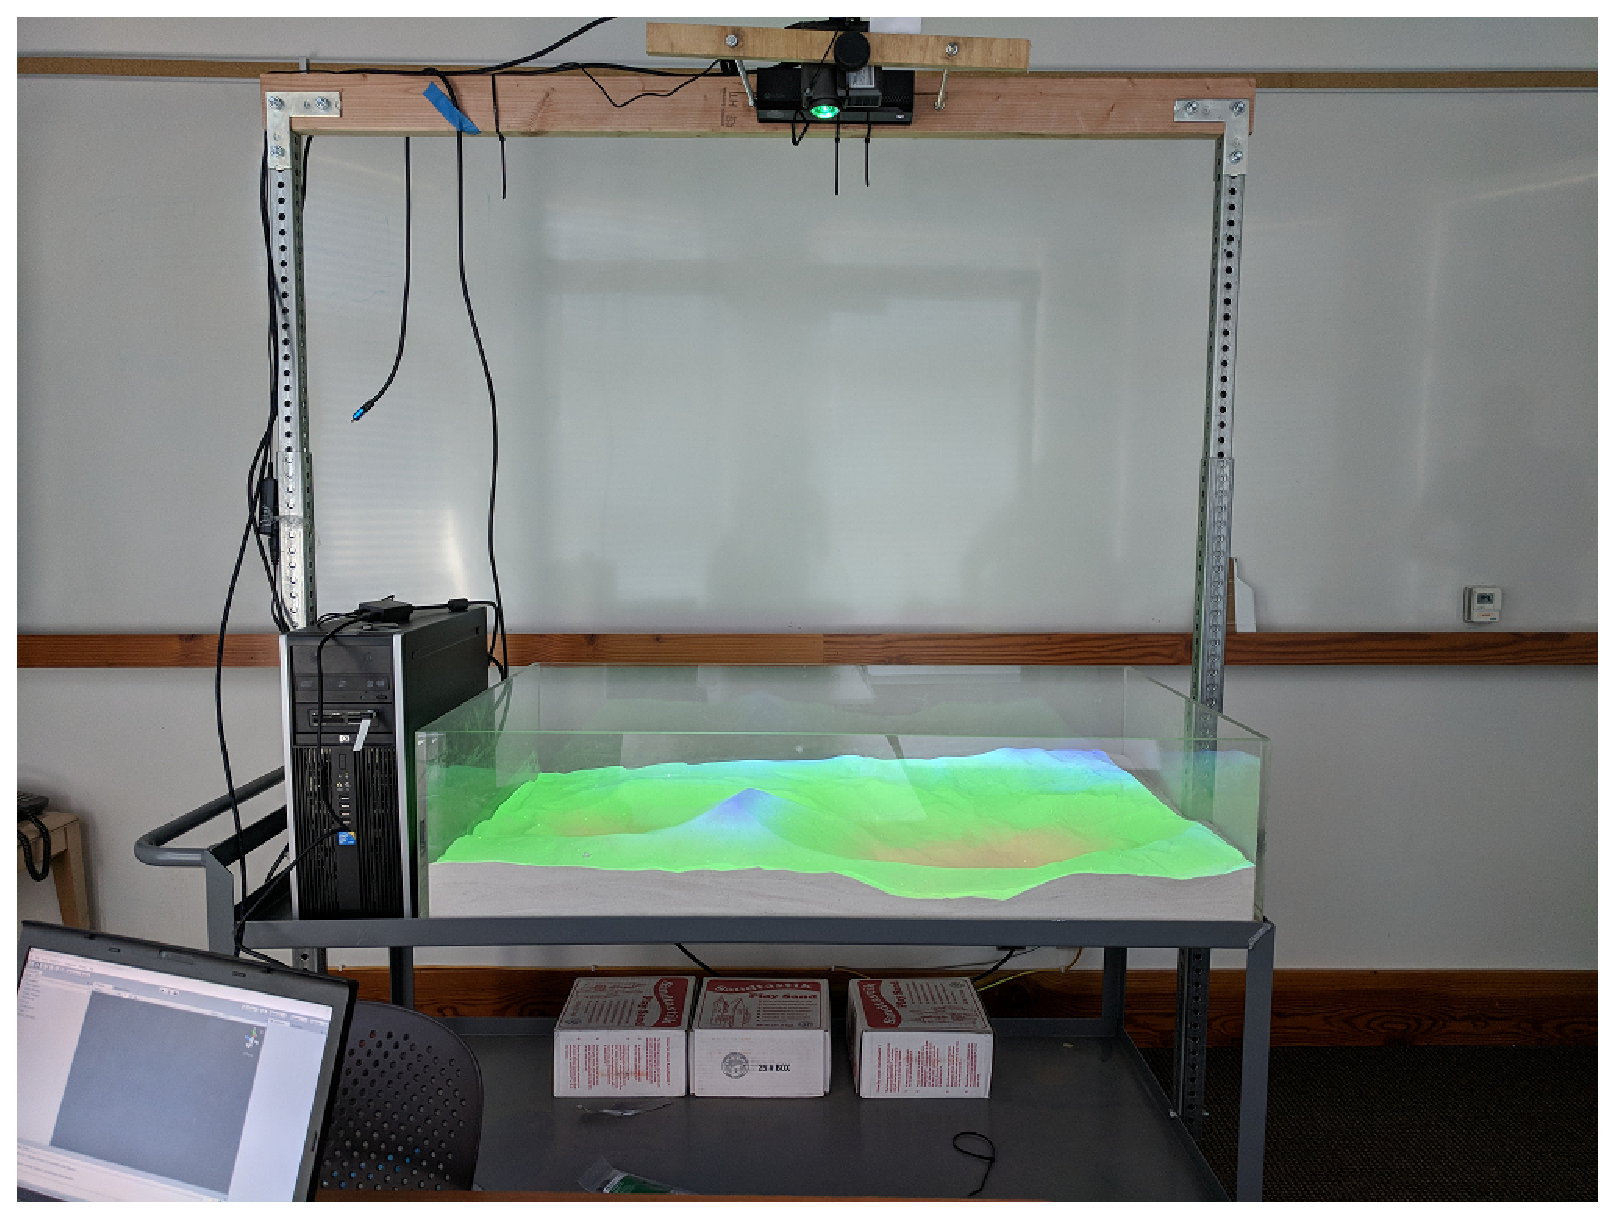
\includegraphics[width=1.\textwidth]{ar_sandbox}
	\caption{A picture of our finished AR sandbox.}
	\label{fig:ar_sandbox}
\end{figure}

\end{appendices}

\end{document}
